\documentclass[a4paper,12pt,oneside,openright]{report}

% this is for dealing with the Too many math alphabets used in version normal" compiling error
\newcommand\hmmax{0} 
\newcommand\bmmax{0}
%%%
\usepackage[spanish]{babel}
\usepackage[utf8]{inputenc}
\usepackage[T1]{fontenc}
\usepackage[x11names,dvipsnames]{xcolor}
\usepackage{amssymb}
\usepackage{amsmath}
\usepackage{verbatim}
\usepackage{booktabs}
\usepackage{multicol}
\usepackage{xspace}
\usepackage{underscore}
\usepackage{upgreek}
% \usepackage[textsize=scriptsize]{todonotes}
\usepackage{lineno}
\usepackage{pxfonts}
\usepackage{algorithm}
\usepackage{algpseudocode}
\floatname{algorithm}{Algoritmo}
\usepackage{bm}
\usepackage{mathtools}
\usepackage[normalem]{ulem}
\usepackage[draft]{fixme}
\usepackage{comment}
\usepackage{url}
\usepackage{graphicx}

\usepackage[font=small,skip=0pt]{caption}

%------------------------------------------------------------------------------------------------


\usepackage{hyperref}

\hypersetup{
  %pdftitle          = {\titulo},
  pdfstartview      = {FitH},
  pdfpagelayout     = {OneColumn},
  plainpages        = false,            % page anchors with formatted form of the page number (i.e., different anchors for pages 'ii' and '2')
  bookmarksnumbered = {true},
  naturalnames      = {true},
  colorlinks        = {true},           % ligas con color; si es falso pone un recuadro que no aparece en la impresion
  linkcolor         = blue,             % color de las ligas dentro del documento (tabla de contenido, secciones, etc.)
  anchorcolor       = red,              % ?
  urlcolor          = NavyBlue,         % color de las ligas externas
  citecolor         = BrickRed          % color de las referencias
}

% para la tabla de contenido
\setcounter{tocdepth}{2}
\setcounter{secnumdepth}{2}

%------------------------------------------------------------------------------------------------


\usepackage{macros}

%Overfull
\overfullrule=0pt
\emergencystretch=1em
% \sloppy
\begin{document}

\title{Algoritmos de Bisimulación para Lógica Knowing How Basada en Incertidumbre}

\author{Antonio Mondejar}

\maketitle

{\hypersetup{linkcolor=black}%
\tableofcontents}
\cleardoublepage

% \section{Marco Teórico: Lógica `Knowing How' Multi-Agente Basada en la Incertidumbre}
\chapter{Lógica de `Knowing How' Multi-Agente Basada en Incertidumbre}
Introduciremos un enfoque para modelar el concepto de saber cómo, presentado en \cite{ArecesFSV25,SaraviaPHD}, el cuál surge a partir de la 
lógica de `Knowing How' previamente introducida en \cite{Wang15KH, Wang2018GoalDirectedKH}. En este enfoque, el conocimiento de un agente está 
representado en Sistemas de Transición Etiquetados (\lts por sus siglas en inglés), donde las transiciones etiquetadas representan el cambio de estado 
que produce cada acción que el agente puede realizar. A su vez, las habilidades de un agente estarán dadas no solo por las acciones básicas que tiene a 
su disposición en un determinado estado, sino que también por la composición de las mismas, es decir, cada camino en el \lts. A las composiciones de acciones las 
llamaremos planes. Se considera que un agente `conoce' un plan en un determinado estado cuando cada ejecución parcial del plan a partir de dicho estado se puede 
completar.

La lógica de `Knowing How' multi-agente basada en incertidumbre toma este enfoque como punto de partida. La principal motivación por la que 
surge esta propuesta es que la representación del conocimiento mencionada anteriormente supone que el agente cuenta con cierto nivel de omnisciencia, 
pues se asume que un agente conoce todo plan que pueda inferirse de su \lts asociado y que, además, sabe distinguir qué plan es adecuado entre los que tiene en su 
disposición, en el sentido de que para todo par de planes es capaz de reconocer si provocan resultados diferentes.
Para clarificar un poco más este argumento, veamos el siguiente ejemplo presentado en \cite{ArecesFSV25,SaraviaPHD}.

Consideremos un agente que quiere hacer una torta. El agente cuenta con la habilidad de realizar cualquiera de los cuatro métodos de mezcla diferentes 
(de batido, de la crema, de fusión y de frotamiento) y hasta podría ser capaz de identificarlos como acciones distintas entre sí. Sin embargo, 
el agente podría no tener noción de cuáles son los efectos de utilizar un método u otro, es decir, podría no distinguir que los mismos producen resultados 
diferentes. En este caso, podríamos considerar que el agente no sabe cómo hacer una torta, pues en los casos en los que selecciona el método correcto obtiene 
un buen resultado y en los demás casos no. 

Incluso, podríamos considerar más situaciones en las que la indistinguibilidad del agente no sea únicamente en acciones sino que en planes en su totalidad. Por ejemplo, 
el agente sabe la diferencia entre añadir leche y añadir harina a la mezcla, pero podría darse el caso en el que no sepa distinguir cuál es el orden adecuado en el que 
realizar ambas acciones. Incluso, podría ocurrir que el agente no sepa distinguir planes de distinta longitud, por ejemplo, en el proceso de horneado de la torta el agente 
debe eventualmente abrir el horno para verificar si el proceso de horneado ya está completo, pero hacerlo con demasiada frecuencia podría afectar al resultado de la torta.

Es así como estos ejemplos motivan una representación más general sobre el conocimiento de un agente, tomando en consideración no solo las habilidades con las que dispone sino 
también su capacidad de distinguir diferentes planes. A su vez, esto permite una representación para múltiples agentes, en la que todos los agentes disponen de las mismas acciones 
pero cada uno tiene su propia interpretación de los efectos de las mismas, así como su propia habilidad para distinguir distintos planes.

Así, la estrategia utilizada en \cite{ArecesFSV25,SaraviaPHD} consiste en fijar un conjunto de agentes $\AGT$ y dotar a los \lts con una 
relación de indistinguibilidad sobre planes para cada agente.

Ahora si, introduciremos la lógica de `Knowing-How' multi-agente basada en incertidumbre (\KHilogic) definiendo su sintaxis y semántica, su noción de bisimulación y por último mencionaremos 
algunos resultados relacionados a su complejidad computacional con respecto a los problemas de verificación de modelos y satisfacibilidad.

\section{Sintaxis y Semántica}
Consideraremos a $\PROP$ como un conjunto no vacío de variables proposicionables con cardinalidad contable 
y a $\AGT$ como un conjunto finito no vacío de nombres de agentes.

\begin{definicion}
    El lenguaje \KHilogic está compuesto por las fórmulas dadas por la gramática:
    \begin{center}
        $\varphi ::= p \mid \neg \varphi \mid \varphi \vee \varphi \mid \varphi \wedge \varphi \mid \kh_i(\varphi,\varphi)$,
    \end{center}
    donde $p \in \PROP$ e $i \in \AGT$. Las constantes booleanas son definidas de la forma usual. Las fórmulas de la forma 
    $\kh_i(\psi, \varphi)$ deben ser leídas como ``cuando vale $\psi$, el agente $i$ sabe cómo hacer que $\varphi$ valga''.
\end{definicion}

Formalizaremos matemáticamente algunos de los conceptos discutidos en la presentación de este capítulo. Como mencionamos, se 
utilizarán secuencias de acciones, o planes, para representar el conocimiento de los agentes. Las fórmulas de \KHilogic se interpretarán 
sobre sistemas de transiciones etiquetados extendidos con una familia de relaciones de indistinguibilidad entre planes.

\begin{definicion}[Acciones y planes]
    Sea $\ACT$ un conjunto enumerable de nombres de acciones, y sea $\ACT^*$ el conjunto de secuencias finitas sobre $\ACT$. 
    A los elementos de $\ACT^*$ los llamaremos planes, siendo $\epsilon$ el plan vacío. Sea $\sigma \in \ACT^*$, denotaremos $|\sigma|$ 
    al largo de $\sigma$ (notar $|\epsilon| = 0$). Para un plan $\sigma$ y $0 \leq k \leq |\sigma|$, el plan $\sigma[..k]$ es el prefijo 
    de $\sigma$ hasta la $k-$ésima posición inclusive. Para $0 < k \leq |\sigma|$, la acción $\sigma[k]$ es la que se encuentra en la 
    $k-$ésima posición de $\sigma$.  
\end{definicion}

\begin{definicion}[Sistemas de Transiciones Etiquetados]
    Un \emph{Sistema de Transición Etiquetado (\lts, Labeled Transition System)} sobre $\PROP$ es una tupla $\modlts = \tup{\W, \R, \V, \ACT}$ 
    donde $\W$ es un conjunto no vacío de estados, $\R = \{\R_a \subseteq \W \times \W \mid a \in A$ para algún $A \subseteq \ACT\}$ es 
    una colección de relaciones binarias sobre $\W$, $\V : \W \to \mathcal{P}(\PROP)$ es una función de etiquetado y $\ACT$ es un 
    conjunto enumerable de nombres de acciones.
\end{definicion}

Gráficamente, un \lts se representa como un grafo dirigido etiquetado, donde los nodos serán los elementos de $\W$, cada uno marcado con las variables proposicionales 
dadas por la función de etiquetado $\V$ y las aristas entre dos nodos estarán dadas por los pares de $\R_a$ para cada $a \in \ACT$.

\begin{ejemplo}\label{ejemplo:lts}
    Sea $\modlts = \tup{\W, \R, \V, \ACT}$ un \lts con:
    
    \begin{itemize}
        \item $\W = \{w_1, w_2, w_3, w_4\}$.
        \item $\R = \{R_a, \R_b\}$ con $\R_a = \{(w_1,w_3), (w_1,w_4), (w_2,w_3)\}$ y $\R_b = \{(w_3,w_4)\}$.
        \item $\V = \{(w_1, \{p\}), (w_2, \{p\}), (w_3, \{q\}), (w_4, \{r\})\}$.
        \item $\ACT = \{a, b\}$.
    \end{itemize}

    Su representación gráfica es (\Cref{fig:lts}):
    \begin{figure}[h]
        \centering
        \begin{tikzpicture}
            \node[state] (p) {$p$};
            \node[state, below of=p, yshift=-1.5cm] (p2) {$p$};
            \node[state, right of=p, yshift=-1cm, xshift=1.5cm] (q) {$q$};
            \node[state, right of=q, xshift=1.5cm] (r) {$r$};
            
            \node at ($(p)+(0,0.5)$) {$w_1$};
            \node at ($(r)+(0,0.5)$) {$w_2$};
            \node at ($(q)+(0,0.5)$) {$w_3$};
            \node at ($(p2)+(0,-0.6)$) {$w_4$};

            \path (p) edge node [above] {$a$} (q)
                      edge [bend left] node [above] {$a$} (r);
            \path (p2) edge node [above] {$a$} (q);
            \path (q) edge node [above] {$b$} (r);
        \end{tikzpicture}
        \caption{Representación gráfica de $\modlts$}
        \label{fig:lts}
    \end{figure}

\end{ejemplo}


\begin{definicion}[\lts basado en incertidumbre]
    Un \emph{\lts-multi-agente basado en incertidumbre (\ults)} sobre $\PROP$ y $\AGT$ es una tupla $\model = \tup{\W,\R,\sim,\V,\ACT}$ 
    donde $\tup{\W,\R,\V,\ACT}$ es un \lts y $\sim$ asigna a cada $i \in \AGT$ una relación de equivalencia sobre un conjunto de planes
    $P_i \subseteq \ACT^*$, también llamada relación de indistinguibilidad. Dado un \ults $\modults$ y $w \in \W$, se llamará 
    al par $(\modults,w)$ un \ults punteado y, usualmente, los paréntesis serán omitidos.
\end{definicion}

Notar que para cada agente $i \in \AGT$, $P_i$ representará los planes que el agente tiene a su disposición. 
Luego $\sim_i$ será una relación de equivalencia sobre $P_i$, donde dos planes estarán relacionados cuando un agente no sepa distinguirlos.

Sea $\model = \tup{\W,\R,\sim,\V,\ACT}$ un \ults y sea $i \in \AGT$, para un plan $\sigma \in P_i$, sea $[\sigma]_i$ su clase de 
equivalencia en $\sim_i$. Notar que hay una correspondencia uno-a-uno entre cada $\sim_i$ y la partición de $P_i$ en sus correspondientes 
clases de equivalencia $\S_i := \{[\sigma]_i \mid \sigma \in P_i\}$. Por lo tanto, de ahora en adelante nos referiremos a los \ults como
una tupla $\tup{\W,\R,\{\S_i\}_{i \in \AGT},\V,\ACT}$.

La representación gráfica de los \ultss será similar a la presentada para los \ltss, con la inclusión de la relación de indistinguibilidad 
entre planes de cada agente.

\begin{ejemplo}\label{ejemplo:ults}
    Siguiendo el \Cref{ejemplo:lts} y considerando $\AGT = \{i\}$, la representación gráfica 
    de $\model=\tup{\W,\R,\{\S_i\}_{i\in\AGT},\V,\ACT}$ es (\Cref{fig:ults}):
    \begin{figure}[h]
        \centering
            \begin{tikzpicture}
                \node[state] (p) {$p$};
                \node[state, below of=p, yshift=-1.5cm] (p2) {$p$};
                \node[state, right of=p, yshift=-1cm, xshift=1.5cm] (q) {$q$};
                \node[state, right of=q, xshift=1.5cm] (r) {$r$};
                
                \node at ($(p)+(0,0.5)$) {$w_1$};
                \node at ($(r)+(0,0.5)$) {$w_2$};
                \node at ($(q)+(0,0.5)$) {$w_3$};
                \node at ($(p2)+(0,-0.6)$) {$w_4$};

                \path (p) edge node [above] {$a$} (q)
                edge [bend left] node [above] {$a$} (r);
                \path (p2) edge node [above] {$a$} (q);
                \path (q) edge node [above] {$b$} (r);
            \end{tikzpicture}
            \hspace{1cm}
            \raisebox{1.8cm}{
                \begin{minipage}{0.45\textwidth}
                    $\S_i = \left\{
                        \begin{array}{c}
                            \{ab,a\}, \{b\}
                        \end{array}
                    \right\}$
                \end{minipage}
            }
            \caption{Representación gráfica de $\modults$}
            \label{fig:ults}
    \end{figure}

    En este caso, los planes que el agente $i$ tiene a su disposición son $\{ab,a,b\}$ y, lo que nos dice su relación de 
    indistinguibilidad $\S_i$ es que a los planes $ab$ y $a$ no sabe distinguirlos.
\end{ejemplo}

Dada entonces la incertidumbre de un agente sobre $\ACT^*$, sus habilidades dependerán no solo de lo que un solo plan puede lograr, sino que de 
lo que cada clase de equivalencia dentro de su relación de indistinguibilidad pueda garantizar.

\begin{definicion}
    Sea $\{\R_a \subseteq \W \times \W \mid a \in A,$ para algún $A \subseteq \ACT \}$ una colección de relaciones binarias sobre $\W$. 
    Se define $\R_\epsilon := \{(w,w) \mid w \in \W\}$ y, para $\sigma \in \ACT^*$ y $a \in \ACT$, 
    $\R_{\sigma a} := \{(w,v) \in \W \times \W \mid$ existe $u \in \W$ tal que $(w,u) \in \R_\sigma$ y $(u,v) \in \R_a \}$. 
    Luego sea $u \in \W$ y $\sigma \in \ACT^*$, se define $\R_\sigma(u) := \{v\in\W \mid (u,v) \in \R_\sigma\}$, y para $U\subseteq\W$ 
    definimos $\R_\sigma(U) := \bigcup\limits_{u \in U} \R_\sigma(u)$.

    Sea $\pi \subseteq \ACT^*$, $u \in \W$ y $U \subseteq \W$, se define
    \[
        \R_\strategy := \bigcup_{\sigma \in \strategy} \R_{\sigma},
    \qquad
        \R_{\strategy}(u) := \bigcup_{\sigma \in \strategy} \R_\sigma(u),
    \qquad
        \R_{\strategy}(U) := \bigcup_{u \in U} \R_{\strategy}(u).
    \]
\end{definicion}

\begin{ejemplo}
    Siguiendo con el \ults presentado en \Cref{ejemplo:ults}, tenemos:
    \begin{itemize}
        \item $\R_{ab} = \{(w_1,w_4), (w_2, w_4)\}$.
        \item $\R_{ab}(w_1) = \{w_4\}$, \quad $\R_{ab}(w_3) = \emptyset$. 
        \item $\R_{a}(\{w_1,w_2\}) = \R_a(w_1) \cup \R_a(w_2) = \{w_3,w_4\} \cup \{w_3\} = \{w_3, w_4\}$.
        \item $\R_{\{ab,b\}} = \R_{ab} \cup \R_b = \{(w_1,w_4),(w_2,w_4),(w_3,w_4)\}$.
        \item $\R_{\{ab,b\}}(w_1) = \R_{ab}(w_1) \cup \R_b(w_1) = \{w_3,w_4\} \cup \emptyset = \{w_3,w_4\}$.
        \item $\R_{\{ab,b\}}(\{w_1,w_3\}) = \R_{\{ab,b\}}(w_1) \cup \R_{\{ab,b\}}(w_3) = \{w_3,w_4\} \cup \{w_4\} = \{w_3,w_4\}$.
    \end{itemize}
\end{ejemplo}


La idea presentada en \cite{ArecesFSV25,SaraviaPHD} consiste en que un agente sabe cómo lograr que valga $\varphi$ dado que vale $\psi$ cuando exista un 
conjunto de planes `adecuado' que pueda ejecutar desde cualquier estado en el que valga $\psi$ y que lleve sólo a estados donde valga $\varphi$. 
Una parte crucial entonces es determinar qué se considerará un conjunto de planes `adecuado'.

\begin{definicion}[Ejecutabilidad Fuerte]
    Sea $\{\R_a \subseteq \W \times \W \mid a \in A$, para algún $A \subseteq \ACT\}$ una colección de relaciones binarias. Un plan $\sigma \in \ACT^*$
    es fuertemente ejecutable ($\sexec$) en un estado $w \in \W$ si y sólo si $\R_\sigma$ está definido y, a su vez, $v \in \R_{\sigma[..k]}(w)$ implica que 
    $\R_{\sigma[k+1]}(v) \neq \emptyset$ para cada $k \in \{0,...,|\sigma|-1\}$. Se define el conjunto $\sexec$($\sigma$) $:= \{w \in \W \mid \sigma$ es $\sexec$ en $w\}$.
    
    Un conjunto de planes $\pi \subseteq \ACT^*$ es fuertemente ejecutable en un estado $u \in \W$ si y sólo si cada $\sigma \in \pi$ es fuertemente ejecutable en $u$.
    Por último, $\sexec$($\pi$) $:= \cap_{\sigma \in \pi}$ $\sexec$($\sigma$) es el conjunto de estados en $\W$ donde $\pi$ es fuertemente ejecutable. 
\end{definicion}

Intuitivamente, ejecutabilidad fuerte sobre planes pide que cada ejecución parcial de un plan (incluyendo $\epsilon$) pueda ser completada, y, ejecutabilidad fuerte sobre
clases de planes pide que cada plan de la clase sea fuertemente ejecutable.

\begin{ejemplo}
    Si consideramos el \ults presentado en \Cref{ejemplo:ults} entonces tenemos que:
    \begin{itemize}
        \item $\sexec(a) = \{w_1,w_2\}$,
        \item $\sexec(ab) = \{w_2\}$, 

        Notar que, a pesar de que $\R_{ab}(w_1) \neq \emptyset$, el plan $ab$ no es fuertemente ejecutable en $w_1$ 
        dado que existe una ejecución parcial que no puede ser completada, pues notar que al tomar la arista 
        $(w_1,w_4)$ con etiqueta $a$ no existe arista con etiqueta $b$ desde $w_4$ para completar el camino.
        \item $\sexec(\{a,ab\}) = \sexec(a) \cap \sexec(ab) = \{w_1,w_2\} \cap \{w_2\} = \{w_2\}$.
    \end{itemize}
\end{ejemplo}


Ahora si, estamos en condiciones de presentar la relación de satisfacibilidad que relaciona \ultss punteados con formulas de \KHilogic. 

\begin{definicion}[\KHilogic sobre \ultss]
    La relación $\models$ entre un \ults punteado $\modults,w$ (con $\model = \tup{\W,\R,\{S_i\}_{i\in\AGT},\V,\ACT})$ y las fórmulas de \KHilogic está definida inductivamente 
    de la siguiente forma:

    \begin{nscenter}
    \sloppy
    \begin{tabular}{@{}l@{\;\;\;}c@{\;\;\;}l@{}}
        $\modults,w \models p$ & \iffdef & $p\in\V(w)$, \\
        $\modults,w \models \neg\varphi$ & \iffdef & $\modults,w \not\models\varphi$, \\ 
        $\modults,w \models \varphi\vee\psi$ & \iffdef & $\modults,w \models \varphi \,\mbox{ o }\, \modults,w \models\psi$, \\
        $\modults,w \models \khi(\psi,\varphi)$ & \iffdef & \begin{minipage}[t]{0.68\textwidth}
                                                         existe $\strategy \in \S_i$ tal que \\
                                                         {\centering
                                                           \begin{inline-cond-kh}\item $\truthset{\modults}{\psi} \subseteq \sexec(\strategy)$ y \item $\R_\strategy(\truthset{\modults}{\psi}) \subseteq \truthset{\modults}{\varphi}$,\end{inline-cond-kh}
                                                          }
                                                       \end{minipage}
    \end{tabular}
    \end{nscenter}
    donde $\truthset{\modults}{\varphi} := \{w \in \W \mid \modults,w \models \varphi\}$. El conjunto de planes $\pi$ en la claúsula semántica de $\khi(\psi,\varphi)$ es llamado
    el testigo de $\khi(\psi,\varphi)$ en $\modults$.
\end{definicion}


Notar que $\khi(\psi,\varphi)$ vale en un estado $w$ cuando existe un conjunto de planes $\pi$ que el agente $i$ considera indistinguibles, tal que al ejecutar cualquier plan $\sigma \in \pi$ a partir de un estado donde vale $\psi$,
toda ejecución parcial puede ser completada terminando en un estado donde vale $\varphi$. También, cabe destacar que como $w$ no tiene ningún rol en la cláusula semántica de $\khi$,
dicho operador actúa \emph{globalmente}. Por lo tanto, $\truthset{\modults}{\khi(\psi,\varphi)}$ es $\W$ o $\emptyset$.

\begin{ejemplo}
    Nuevamente, consideremos el \ults presentado en \Cref{ejemplo:ults}, y veamos que:
    \begin{itemize}
        \item $\modults,w_1 \models p$ pero $\modults,w_3 \not\models p$.
        \item Notemos que $\sexec(\{ab,a\}) = \{w_2\}$ y $\sexec(\{b\}) = \{w_3\}$. 
        Luego $\truthset{\modults}{p} = \{w_1,w_2\} \not\subseteq \sexec(\pi)$ para todo $\pi \in \S_i$.
        Por lo que podemos afirmar que $\modults,w_1 \not\models \khi(p,q)$.
        Más aún, $\modults,w_j \not\models \khi(p,q)$ para cada $j \in \{1,..,4\}$.
        \item Como mencionamos en el item anterior, $\sexec(\{b\}) = \{w_3\}$. Luego, podemos ver que 
        $\modults, w_1 \models \khi(q,r)$ y $\{b\} \in \S_i$ es su testigo. 
        Pues, $\truthset{\modults}{q} = \{w_3\} \subseteq \sexec(\{b\})$ y $\R_b(w_3) = \{w_4\} \subseteq \truthset{\modults}{r}$.         

        A su vez, por la globalidad de $\khi$, ocurre que $\modults,w_j \models \khi(q,r)$ para cada $j \in \{1,...,4\}$.
    \end{itemize}
\end{ejemplo}



\section{Bisimulación}

La bisimulación es una herramienta crucial a la hora de analizar el poder expresivo de una lógica o un lenguaje formal. 
Nos permite relacionar modelos a partir de características estructurales entre sí, las cuáles logran capturar el comportamiento de 
los mismos con respecto a la lógica en cuestión. 

Se presentará aquí su definición junto con algunos resultados deseables a la hora de estudiar la noción de bisimulación de una 
lógica modal, los cuáles fueron demostrados en \cite{ArecesFSV25,SaraviaPHD}.

Primero, introduciremos una notación que nos será útil.

\begin{definicion}
    Sea $\model=\tup{\W,\R,\cset{\S_i}_{i \in \AGT},\V,\ACT}$ un \ults sobre $\PROP$ y $\AGT$.

    Tomemos un conjunto de planes $\pi \subseteq \ACT^*$, un conjunto de estados $U \subseteq \W$ y un agente $i \in \AGT$.
    \begin{itemize}
        \item Escribiremos $U \ultsExecStrat{\pi} T$ $\iffdef$ $U \subseteq \sexec(\pi)$ y $\R_\pi(U) \subseteq T$.
        \item Escribiremos $U \ultsExecAgi T$ $\iffdef$ existe $\pi \in \S_i$ tal que $U \ultsExecStrat{\pi} T$.
    \end{itemize}
    A su vez, decimos que $U \subseteq \W$ es \KHilogic-definible en $\modults$ si y sólo si existe una \KHilogic-fórmula $\varphi$ tal que
    $U = \truthset{\modults}{\varphi}$. Análogamente, decimos que $U \subseteq \W$ es proposicionalmente definible en $\modults$ 
    si y sólo si existe una fórmula proposicional $\varphi$ tal que $U = \truthset{\modults}{\varphi}$.
\end{definicion}

Una observación que surge de esta definición es que si un conjunto es proposicionalmente definible entonces es \KHilogic-definible, dado que 
toda fórmula proposicional sobre $\PROP$ es también una \KHilogic-fórmula.

La siguiente proposición presentada en \cite{ArecesFSV25,SaraviaPHD} nos dice que también vale la recíproca, 
es decir, que si un conjunto es \KHilogic-definible entonces es proposicionalmente definible.

\begin{proposicion}\label{prop:khi-implies-prop-definable}
    Sea $\model=\tup{\W,\R,\cset{\S_i}_{i \in \AGT},\V,\ACT}$ un \ults. Para todo $U \subseteq \W$, si $U$ es \KHilogic-definible, entonces $U$ es proposicionalmente definible.
\end{proposicion}

Ahora si, presentamos la noción de bisimulación.

\begin{definicion}[\KHilogic-bisimulación]\label{def:bisimulation}
    Sean $\modults$ y $\modults'$ dos \ultss, con dominios $\W$ y $\W'$ respectivamente. Sea $Z \subseteq \W \times \W'$.
    \begin{itemize}
        \item Sea $u \in W$ y $U \subseteq \W$, definimos
        \begin{nscenter}
            \begin{tabular}{@{}c@{}}
                $Z(u) := \csetsc{u' \in \W'}{(u,u') \in Z}$, \qquad $Z(U) := \bigcup_{u \in U} Z(u)$.
            \end{tabular}
        \end{nscenter}
        \item Sea $u' \in \W'$ y $U' \subseteq \W'$, definimos
        \begin{nscenter}
            \begin{tabular}{@{}c@{}}
                $Z^{-1}(u') := \csetsc{u \in \W}{(u,u') \in Z}$; \qquad $Z^{-1}(U') := \bigcup_{u' \in U'} Z^{-1}(u')$.
            \end{tabular}
        \end{nscenter}
    \end{itemize}

    Una relación binaria no vacía $Z \subseteq \W \times \W'$ es llamada una \KHilogic-bisimulación entre $\modults$ y 
    $\modults'$ si y sólo si $(w,w') \in Z$ implica lo siguiente:
    \begin{itemize}
        \item \textbf{Atom}: $\V(w)=\V'(w')$.

        \item \textbf{$\khi$-zig}: para cada conjunto \emph{proposicionalmente} definible $U \subseteq \W$, si $U \ultsExecAgi T$ para algún $T \subseteq \W$, entonces existe $T' \subseteq \W'$ tal que
        \begin{multicols}{2}
            \begin{cond-bisim}
                \item $Z(U) \ultsExecAgi T'$, 
                \item $T' \subseteq Z(T)$.
            \end{cond-bisim}
        \end{multicols}
        
        \item \textbf{$\khi$-zag}: para cada conjunto \emph{proposicionalmente} definible $U' \subseteq \W'$, si $U' \ultsExecAgi T'$ para algún $T' \subseteq \W'$, entonces existe $T \subseteq \W$ tal que
        \begin{multicols}{2}
            \begin{cond-bisim}
                \item $Z^{-1}(U') \ultsExecAgi T$,
                \item $T \subseteq Z^{-1}(T')$.
            \end{cond-bisim}
        \end{multicols}

        \item \textbf{A-zig}: para cada $u \in \W$ existe $u' \in \W'$ tal que $(u,u') \in Z$.

        \item \textbf{A-zag}: para cada $u' \in \W'$ existe $u \in \W$ tal que $(u,u') \in Z$.
    \end{itemize} 

    Escribiremos $\modults,w \bisim \modults',w'$ cuando exista una \KHilogic-bisimulación $Z$ entre
    $\modults$ y $\modults'$ tal que $(w,w') \in Z$.
\end{definicion}

Para poder formalizar las propiedades cruciales de la bisimulación, definiremos primero la noción de 
equivalencia entre modelos con respecto a \KHilogic.

\begin{definicion}[\KHilogic-equivalencia]
    Dos \ultss punteados $\modults,w$ y $\modults',w'$ son \KHilogic-equivalentes ($\model, w \modequiv \model', w'$)
    si y sólo si, para cada $\varphi \in \KHilogic$,
    \begin{center}
        $\model, w \models \varphi$ \quad si y sólo \quad $\model', w' \models \varphi$.
    \end{center} 
\end{definicion}

Ahora, podemos presentar la correspondencia esperada entre $\bisim$ y $\modequiv$, demostrada en \cite{ArecesFSV25,SaraviaPHD}.
Usualmente nos referimos a este resultado como el Teorema de Invarianza para Bisimulación.

\begin{teorema}[\KHilogic-bisimilitud implica \KHilogic-equivalencia]\label{thm:bisim-implies-equivalence}
    Sean $\modults,w$ y $\modults',w'$ dos \ultss punteados, entonces
    \begin{center}
        $\modults,w \bisim \modults',w'$ implica $\modults,w \modequiv \modults',w'$.
    \end{center}
\end{teorema}

Este teorema caracteriza a la bisimulación como una noción que permite relacionar modelos \KHilogic-equivalentes, es decir, que la lógica no tiene una fórmula con la cuál distinguirlos,
a partir de propiedades puramente estructurales de los mismos.

En \cite[Sección 2]{FervariVQW21} se presenta un contraejemplo que atestigua que la recíproca del \Cref{thm:bisim-implies-equivalence} 
no es cierta para cualquier par de modelos. Un problema ampliamente estudiado en la literatura de las lógicas modales es el de analizar 
en qué clases de modelos vale la recíproca del teorema, dichas clases son conocidas como clases de Hennessy-Milner.
En \cite{ArecesFSV25,SaraviaPHD}, se demuestra que la clase de \ults finitos es una clase de Hennessy-Milner, es decir, satisface la 
recíproca de \Cref{thm:bisim-implies-equivalence}.

Diremos que $\modults$, un \ults, es finito si y sólo si cada una de sus componentes tiene cardinalidad finita. Análogamente, diremos que 
($\modults,w$), un \ults punteado, es finito si y sólo $\modults$ es finito. 

\begin{teorema}[\KHilogic-equivalencia implica \KHilogic-bisimilitud]\label{thm:finite-equivalence-implies-bisim}
    Sean $\modults,w$ y $\modults',w'$ dos \ultss punteados finitos, entonces
    \begin{center}
        $\model,w \modequiv \model', w'$ implica $\model,w \bisim \model', w'$.
    \end{center}
\end{teorema}

Notemos que este teorema es un gran resultado en términos computacionales. Como los algoritmos trabajan siempre con modelos finitos, este resultado
nos dice que si se consigue un procedimiento efectivo que decida bisimilitud entre dos \ultss punteados, dicho procedimiento estará decidiendo a la vez
equivalencia lógica entre los \ultss punteados en cuestión.


\section{Complejidad Computacional}

A lo largo de este trabajo, analizaremos la complejidad computacional de problemas relacionados con la noción de bisimulación. 
Por ello, vale la pena mencionar algunos resultados estudiados en \cite{ArecesFSV25,SaraviaPHD} referentes a la lógica presentada en este 
capítulo. 

A la hora de realizar un estudio computacional de una lógica, los dos problemas de decisión fundamentales a analizar son los de 
verificación de modelos (Model Checking) y satisfacibilidad ($\SAT$).

El problema de Model Checking se formula como "dado un modelo y una fórmula de la lógica, decidir si el modelo la satisface". Por otro lado, 
$\SAT$ se formula como "dada una fórmula de la lógica, decidir si existe un modelo que la satisfaga". 

Estos problemas han sido estudiados a lo largo de los años en numerosas lógicas y son centrales, no solo para la lógica computacional, sino que 
también para la teoría de la complejidad computacional en general. 

Para la lógica proposicional, el problema de Model Checking está en la clase $\Poly$, mientras que $\SAT$ es $\NPComplete$ 
\cite[Capítulo 2, Sección 3]{Goldreich_2008}. Por otro lado, en la lógica modal básica tenemos que Model Checking también 
está en $\Poly$ pero $\SAT$ es $\PSPACEComplete$ \cite[Capítulo 4]{HandbookModalLogic}. En la lógica de primer orden, el problema de 
Model Checking es $\PSPACEComplete$ \cite[Capítulo 5, Sección 4]{Goldreich_2008} y $\SAT$ es indecidible. 

Una observación que surge a partir de estos resultados es que mientras mayor es el poder expresivo de la lógica, mayores son los recursos 
computacionales que se necesitan para resolver ambos problemas.

Metiendonos de lleno en las lógicas de `Knowing How', en \cite{Demri_Fervari_2023} se demostró que para la lógica de `Knowing How' introducida 
en \cite{Wang15KH,Wang2018GoalDirectedKH} Model Checking es $\PSPACEComplete$. Por otro lado, en \cite{SAT_Upper_Bound} se demostró que 
$\SAT \in \NP^{\NP}$, aunque no se ha encontrado todavía una cota inferior de su complejidad computacional.

Para \KHilogic, en \cite{ArecesFSV25,SaraviaPHD} se obtienen los siguientes resultados sobre los problemas de decisión mencionados:
\begin{teorema}
    El problema de Model Checking para \KHilogic está en $\Poly$.
\end{teorema}

\begin{teorema}
    $\SAT$ para \KHilogic es $\NPComplete$.
\end{teorema}

Lo que nos dice que ambos problemas son más fáciles, computacionalmente hablando, en su versión para \KHilogic con respecto a su versión para 
la lógica de `Knowing How' previamente mencionada.

% \section{Redefiniendo la Noción de Bisimulación}
\chapter{Redefiniendo la Noción de Bisimulación}

La noción de bisimulación de una lógica modal nos permite relacionar dos modelos a partir de características puramente estructurales 
que comparten entre sí, con las que se logra garantizar la equivalencia lógica entre ellos. En ese sentido, consideramos que la 
bisimulación modela la idea de equivalencia en cuanto al comportamiento de ambos modelos respecto a una lógica en particular.

Ahora bien, si analizamos la definición presentada en \ref{def:bisimulation}, podemos notar que en ($\khi$-zig) y ($\khi$-zag) se piden condiciones 
sobre los conjuntos proposicionalmente definibles de los dominios de cada modelo, lo cuál naturalmente no es una condición estructural de los modelos, 
ya que dichos conjuntos dependen de la existencia de una fórmula, es decir, un objeto puramente sintáctico de la lógica. 

A su vez, a la hora de presentar una noción de bisimulación, es deseable que la misma tenga una naturaleza `procedural', es decir,
que dada una relación binaria entre los dominios de dos modelos sea posible diseñar un procedimiento efectivo que verifique si dicha relación 
es una bisimulación.

Nuevamente, si analizamos la definicion presentada en la sección anterior, podemos notar que para verificar que una relación binaria es una bisimulación
tenemos que explorar necesariamente los conjuntos proposicionalmente definibles de los dominios de cada modelo, lo cuál lleva consigo una cantidad 
infinita de fórmulas proposicionales que analizar, por lo que no parece una tarea sencilla encontrar un procedimiento efectivo que realice lo deseado.

Es así como surge la motivación de esta sección. Propondremos una nueva noción de bisimulación para la lógica presentada, modificando las condiciones
($\khi$-zig) y ($\khi$-zag) para que sólo se consideren características estructurales de ambos modelos, y, a su vez, se tenga una naturaleza procedural.

Primero veremos algunos lemas para caracterizar los conjuntos proposicionalmente definibles del dominio de un modelo $\modults$.

\begin{lema}\label{ref:propositional-equivalence}
    Sea $\model=\tup{\W,\R,\cset{\S_i}_{i \in \AGT},\V,\ACT}$ un \ults, y sean $w$, $v \in \W$
    tales que $\V(w)$ = $\V(v)$ entonces para toda $\varphi$ proposicional se cumple que, 
    \begin{center}
    $\modults, w \models \varphi$ \quad si y sólo si \quad $ 
    \modults, v \models \varphi$
    \end{center}
\end{lema}

\begin{demostracion}
    Sea $\model=\tup{\W,\R,\cset{\S_i}_{i \in \AGT},\V,\ACT}$ y $w$, $v \in \W$
    tales que $\V(w)$ = $\V(v)$. La demostración es por inducción estructural sobre $\varphi$. 
    Recordar que $\varphi$ es una fórmula \textbf{proposicional}.

    \begin{itemize}
        \item Caso base: $\varphi = p$ donde $p \in \PROP$.

        Notar que  $\modults, w \models \varphi$ si y sólo si $p \in \V(w)$.

        Ahora bien, como $\V(w)$ = $\V(v)$, $p \in \V(w)$ si y sólo si $p \in \V(v)$.

        Finalmente, por la definición de $\models$, $p \in \V(v)$ si y sólo si $\modults, v \models \varphi$.  
    
        \item Caso inductivo: La hipótesis inductiva establece que, para $\psi$ una subfórmula de $\varphi$, 
        se cumple que $\modults, w \models \psi$ si y sólo si $\modults, v \models \psi$.

        \begin{itemize}
            \item Caso $\varphi = \psi_1 \lor \psi_2$. 
    
            Por definición de $\models$, $\modults, w \models \psi_1 \lor \psi_2$ si y sólo si $\modults,
            w \models \psi_1$ o $\modults, w \models \psi_2$.
            
            Por hipótesis inductiva, $\modults, w \models \psi_1$ o $\modults, w \models \psi_2 $ si y sólo
            si $\modults, v \models \psi_1$ o $\modults, v \models \psi_2$. 
            
            Pero notar que, nuevamente por definición de $\models$, $\modults, v \models \psi_1$ o $\modults,
            v \models \psi_2$ si y sólo si $\modults,v \models \psi_1 \lor \psi_2$.  

            \item Caso $\varphi = \neg \psi$.
        
            La demostración es similar a la del caso analizado anteriormente.
        \end{itemize}
    
    \end{itemize}
    
\end{demostracion}

Definiremos para cada modelo una relación de equivalencia sobre su dominio, la cuál particiona a los nodos de acuerdo
a su función de valuación.

\begin{definicion}\label{def:A_m}
    Sea $\model=\tup{\W,\R,\cset{\S_i}_{i \in \AGT},\V,\ACT}$ un \ults entonces se define, 
    \begin{center}
        $A_\modults := \{(w,v) \in \W \times \W \mid \V(w) = \V(v)\}$
    \end{center}
    Notar que $A_\modults$ es una relación de equivalencia sobre $\W$. Luego se denotará,
    \begin{center}
        $\rho_\modults := \{ [w] \mid w \in \W $ y $[w]$ su clase de equivalencia respecto a $A_\modults\}$
    \end{center}
\end{definicion}

Ahora estamos en condiciones de presentar esta propiedad de los conjuntos proposicionalmente definibles del dominio de un modelo $\modults$.

\begin{lema}\label{ref:propositionally-definable-lemma}
    Sea $\model=\tup{\W,\R,\cset{\S_i}_{i \in \AGT},\V,\ACT}$ un \ults y sea $U \subseteq \W$ tal que $U$ es proposicionalmente definible, entonces
    \begin{center}
        para cada $s_i \in \rho_\modults$ se cumple que $s_i \cap U = \emptyset$ o $s_i \subseteq U$.
    \end{center}
\end{lema}

\begin{demostracion}
    $\model=\tup{\W,\R,\cset{\S_i}_{i \in \AGT},\V,\ACT}$ un \ults y sea $U \subseteq \W$ tal que $U$ es proposicionalmente definible, 
    veamos que se cumple la propiedad mencionada.

    Como $U$ es proposicionalmente definible entonces existe $\varphi$ proposicional que lo define.

    Sea $s_i \in \rho_\modults$, notemos que si $s_i \cap U = \emptyset$ entonces la propiedad vale.
    
    Supongamos entonces que $s_i \cap U \neq \emptyset$ y veamos que $s_i \subseteq U$. Como $s_i \cap U \neq \emptyset$, entonces existe 
    $w \in U$ tal que $[w] = s_i$, y como $w \in U$ entonces ocurre que $\modults,w \models \varphi$. Ahora bien, sea $v \in s_i$ 
    entonces sabemos que $\V(v) = \V(w)$, luego por \ref{ref:propositional-equivalence} tenemos que $\modults,v \models \varphi$, por 
    lo que $v \in U$. Lo que nos dice que $s_i \subseteq U$ que era lo que queríamos demostrar.  
\end{demostracion}

A partir de esta propiedad, surge la nueva noción de bisimulación que proponemos para la lógica `Knowing-How' multi-agente basada en la 
incertidumbre.

\begin{definicion}[\KHilogic-bisimulación$^*$]\label{def:bisim_redefinition}
    Sean $\modults$ y $\modults'$ dos \ultss, con dominios $\W$ y $\W'$ respectivamente.
    Una relación binaria no vacía $Z \subseteq \W \times \W'$ es llamada una \KHilogic-bisimulación$^*$ entre $\modults$ y 
    $\modults'$ si y sólo si $(w,w') \in Z$ implica lo siguiente
    \begin{itemize}
        \item \textbf{Atom}: $\V(w)=\V'(w')$.

        \item \textbf{$\khi$-zig$^*$}: Sea $U \subseteq \W$ tal que para cada $s_i \in \rho_\modults$ se cumple que $s_i \cap U = \emptyset$ o $s_i \subseteq U$, si $U \ultsExecAgi T$ para algún $T \subseteq \W$, entonces existe $T' \subseteq \W'$ tal que
        \begin{multicols}{2}
            \begin{cond-bisim}
                \item $Z(U) \ultsExecAgi T'$, 
                \item $T' \subseteq Z(T)$.
            \end{cond-bisim}
        \end{multicols}
        
        \item \textbf{$\khi$-zag$^*$}: Sea $U' \subseteq \W'$ tal que para cada $s_i' \in \rho_{\modults'}$ se cumple que $s_i' \cap U' = \emptyset$ o $s_i' \subseteq U'$, si $U' \ultsExecAgi T'$ para algún $T' \subseteq \W'$, entonces existe $T \subseteq \W$ tal que
        \begin{multicols}{2}
            \begin{cond-bisim}
                \item $Z^{-1}(U') \ultsExecAgi T$,
                \item $T \subseteq Z^{-1}(T')$.
            \end{cond-bisim}
        \end{multicols}

        \item \textbf{A-zig}: para cada $u \in \W$ existe $u' \in \W'$ tal que $(u,u') \in Z$.

        \item \textbf{A-zag}: para cada $u' \in \W'$ existe $u \in \W$ tal que $(u,u') \in Z$.
    \end{itemize} 

    Escribiremos $\modults,w \bisim^* \modults',w'$ cuando exista una \KHilogic-bisimulación$^*$ $Z$ entre
    $\modults$ y $\modults'$ tal que $(w,w') \in Z$.
\end{definicion}

Una vez definida la nueva noción, notemos que \ref{ref:propositionally-definable-lemma} nos permite demostrar de forma casi directa que
toda relación binaria que satisface las nuevas condiciones presentadas de ($\khi$-zig$^*$) y ($\khi$-zag$^*$) también satisface las condiciones
presentadas en \ref{def:bisimulation}.

\begin{lema}[\KHilogic-bisimilitud$^*$ implica \KHilogic-bisimilitud]\label{ref:new_bisim-implies-old_bisim}
    Sean $\modults$ y $\modults'$ dos \ultss, con dominios $\W$ y $\W'$ respectivamente. Si $Z \subseteq \W \times \W'$ es una \KHilogic-bisimulación$^*$ entonces $Z$ es una \KHilogic-bisimulación.
\end{lema}

\begin{demostracion}
    Queremos ver que $Z$ es una \KHilogic-bisimulación.

    Notemos que $Z$ satisface (Atom), (A-zig) y (A-zag) dado que $Z$ es una \KHilogic-bisimulación$^*$.

    Veamos entonces que satisface ($\khi$-zig) y ($\khi$-zag).

    \begin{itemize}
        \item ($\khi$-zig) Sea $U \subseteq \W$ proposicionalmente definible y sea $T \subseteq \W$ tal que $U \ultsExecAgi T$, queremos ver que existe
        $T' \subseteq \W'$ tal que

        \begin{multicols}{2}
            \begin{cond-bisim}
                \item $Z(U) \ultsExecAgi T'$, 
                \item $T' \subseteq Z(T)$.
            \end{cond-bisim}
        \end{multicols}
        Notemos que como $U$ es proposicionalmente definible entonces por \ref{ref:propositionally-definable-lemma}, $U$ satisface que para cada $s_i \in \rho_\modults$ se cumple
        que $s_i \cap U = \emptyset$ o $s_i \subseteq U$.
    
        Luego como $Z$ satisface ($\khi$-zig$^*$) tenemos asegurada la existencia de dicho $T'$.
    
        \item ($\khi$-zag) Análogo a ($\khi$-zig).
    \end{itemize}

    Finalmente hemos demostrado que $Z$ es una \KHilogic-bisimulación.
\end{demostracion}

Ahora bien, notemos como este lema nos permite demostrar el Teorema de Invarianza para nuestra nueva noción de bisimulación.

\begin{teorema}[\KHilogic-bisimilitud$^*$ implica \KHilogic-equivalencia]
    Sean $\modults,w$ y $\modults',w'$ dos \ultss punteados, entonces
    \begin{center}
        $\modults,w \bisim^* \modults',w'$ implica $\modults,w \modequiv \modults',w'$.
    \end{center}
\end{teorema}

\begin{demostracion}
    Sean $\modults,w$ y $\modults',w'$ dos \ultss punteados tales que $\modults,w \bisim^* \modults',w'$, entonces existe $Z$ \KHilogic-bisimulación$^*$
    entre $\modults$ y $\modults'$ tal que $(w,w') \in Z$.
    
    Luego por \ref{ref:new_bisim-implies-old_bisim} sabemos que $Z$ es una \KHilogic-bisimulación, y como $(w,w') \in Z$ entonces $\modults,w \bisim \modults',w'$.

    Finalmente, por \ref{ref:bisim-implies-equivalence}, tenemos que $\modults,w \modequiv \modults',w'$.
\end{demostracion}

Una vez demostrado el Teorema de Invarianza para la noción propuesta, nos gustaría demostrar que también se mantiene la otra dirección en
el caso finito. 

Para lograr esto, primero fortaleceremos la propiedad dada en \ref{ref:propositionally-definable-lemma} para el caso finito.

\begin{lema}\label{ref:finite-propositionally-definable-lemma}
    Sea $\model=\tup{\W,\R,\cset{\S_i}_{i \in \AGT},\V,\ACT}$ un \ults finito y sea $U \subseteq \W$, entonces
    para cada $s_i \in \rho_\modults$ se cumple que $s_i \cap U = \emptyset$ o $s_i \subseteq U$ si y sólo si $U$ es proposicionalmente definible.
\end{lema}

\begin{demostracion}
    Notar que la direccion ($\leftarrow$) está demostrada en \ref{ref:propositionally-definable-lemma}. Entonces demostremos ($\rightarrow$).

    Supongamos que para cada $s_i \in \rho_\modults$ se cumple que $s_i \cap U = \emptyset$ o $s_i \subseteq U$.

    Primero, notemos que como $\modults$ es finito, entonces existen un número finito de variables proposicionales $p_1,...,p_n$ que aparecen en la imagen de $\V$ para algún $w \in \W$.

    Ahora bien, por un lado si $U = \emptyset$, luego la fórmula $ \varphi := \bot$ define a $U$. Entonces supongamos que $U \neq \emptyset$. 
    
    Sea $S = \{s_1,...,s_m\}$ tal que cada $s_i \subseteq U$. Recordar que cada $s_i$ es una clase de equivalencia de la relación $A_\modults$. A su vez, para cada $w$, $v \in s_i$ se cumple que $\V(w) = \V(v)$. Se utilizará $\V(s_i)$ para hacer referencia a $\V(w)$ para cada $w \in s_i$.

    Sea $\varphi_i := \bigwedge\limits_{j = 1}^{n} l_i(p_j)$ donde $l_i(p_j) = $
    $\left\{ \begin{array}{rcl}
            p_j & \mbox{si}
            & p_j \in \V(s_i) \\ \neg p_j & \mbox{si} & p_j \notin \V(s_i) \\
            \end{array}\right. 
    $.

    Veamos que por la forma en la que construimos $\varphi_i$, se cumple que $\modults, w \models \varphi_i$ si y sólo si $w \in s_i$. ($*$)
    
    Demostremos entonces que $\varphi := \bigvee\limits_{i = 1}^{m}\varphi_i$ define a $U$. Primero, notar que sea $w \in \W$, $\modults, w \models \varphi$ si y sólo si $\modults, w \models \varphi_i$ para algún $i \in \{1,...m\}$.  

    Queremos ver entonces que, $w \in U$ si y sólo si $\modults, w \models \varphi$. 

    Sea $w \in U$, por hipótesis, existe $s_i$ tal que $w \in s_i$ y a su vez $s_i \subseteq U$. Pues notar que como $w \in U$ entonces $s_i \cap U \neq \emptyset$, luego necesariamente $s_i \subseteq U$.
    
    Ahora bien, por $(*)$, $\modults, w \models \varphi_i$, por lo que $\modults, w \models \varphi$.

    Sea $w \in \W$ tal que $\modults, w \models \varphi$, entonces existe $i \in \{1,...,m\}$ tal que $\modults, w \models \varphi_i$. Luego por $(*)$, $w \in s_i$, lo que nos dice que $w \in U$.

    Luego $\varphi$ define a $U$.
    
    Como $\varphi$ es proposicional, $U$ es proposicionalmente definible.
\end{demostracion}

De esta lema obtenemos un corolario sobre el problema de determinar si un subconjunto del dominio de un \ults es \KHilogic-definible.

\begin{corolario}[\KHilogic-definibilidad]
    Sea $\model=\tup{\W,\R,\cset{\S_i}_{i \in \AGT},\V,\ACT}$ un \ults finito y sea $U \subseteq \W$, el problema de determinar si $U$ es 
    \KHilogic-definible está en $\Poly$.
\end{corolario}

\begin{demostracion}

    Primero, notemos que determinar si $U$ es \KHilogic-definible es equivalente a determinar si $U$ es proposicionalmente definible, por lo visto en 
    \ref{ref:khi_definable-implies-propositionally_definable}.

    Luego, por \ref{ref:finite-propositionally-definable-lemma}, basta con dar un algoritmo que compute $\rho_\modults$ y para cada $s_i \in \rho_\modults$ 
    chequee que $s_i \subseteq U$ o $s_i \cap U = \emptyset$. Lo cuál es claro que puede realizarse en tiempo polinomial sobre el tamaño de $\modults$.
\end{demostracion}

Ahora bien, notemos como el fortalecimiento de la propiedad sobre los conjuntos proposicionalmente definibles nos permite fortalecer también \ref{ref:new_bisim-implies-old_bisim}.

\begin{lema}[\KHilogic-bisimilitud implica \KHilogic-bisimilitud$^*$]\label{ref:finite-old_bisim-implies-new_bisim}
    Sean $\modults$ y $\modults'$ dos \ultss finitos, con dominios $\W$ y $\W'$ respectivamente. Sea $Z \subseteq \W \times \W'$, entonces 
    \begin{center}
        $Z$ es una \KHilogic-bisimulación$^*$ si y sólo si $Z$ es una \KHilogic-bisimulación.
    \end{center}
\end{lema}

\begin{demostracion}
    Notar que la dirección ($\rightarrow$) está demostrada en \ref{ref:new_bisim-implies-old_bisim}, entonces demostremos ($\leftarrow$).
    
    Sea $Z$ una \KHilogic-bisimulación, veamos que es una \KHilogic-bisimulación$^*$.

    Notemos que $Z$ satisface (Atom), (A-zig) y (A-zag) dado que $Z$ es una \KHilogic-bisimulación.

    Así que demostremos que $Z$ satisface ($\khi$-zig) y ($\khi$-zag).

    \begin{itemize}
        \item ($\khi$-zig) Sea $U \subseteq \W$ tal que para cada $s_i \in \rho_\modults$ se cumple que $s_i \cap U = \emptyset$ o $s_i \subseteq U$ 
        y sea $T \subseteq \W$ tal que $U \ultsExecAgi T$, queremos ver que existe $T' \subseteq \W'$ tal que

        \begin{multicols}{2}
            \begin{cond-bisim}
                \item $Z(U) \ultsExecAgi T'$, 
                \item $T' \subseteq Z(T)$.
            \end{cond-bisim}
        \end{multicols}

        Notemos que como para cada $s_i \in \rho_\modults$ se cumple que $s_i \cap U = \emptyset$ o $s_i \subseteq U$ y $\modults$ es finito entonces 
        por \ref{ref:finite-propositionally-definable-lemma} $U$ es proposicionalmente definible.
    
        Luego como $Z$ satisface ($\khi$-zig$^*$) tenemos asegurada la existencia de dicho $T'$.
    
        \item ($\khi$-zag) Análogo a ($\khi$-zig). 
    \end{itemize}

    Finalmente hemos demostrado que $Z$ es una \KHilogic-bisimulación.
\end{demostracion}

Y como demostramos que en el caso finito ambas nociones de bisimulación son equivalentes, estamos en condiciones de demostrar el teorema deseado. 

\begin{teorema}[\KHilogic-equivalencia implica \KHilogic-bisimilitud$^*$]
    Sean $\modults,w$ y $\modults',w'$ dos \ultss punteados finitos, entonces
    \begin{center}
        $\model,w \modequiv \model', w'$ implica $\model,w \bisim^* \model', w'$.
    \end{center}
\end{teorema}

\begin{demostracion}
    Sean $\modults,w$ y $\modults',w'$ dos \ultss punteados finitos tales que $\model,w \modequiv \model', w'$, entonces por \ref{ref:finite-equivalence-implies-bisim}
    tenemos que $\model,w \bisim \model', w'$. Luego existe $Z$ \KHilogic-bisimulación tal que $(w,w') \in Z$.

    Ahora bien, por \ref{ref:finite-old_bisim-implies-new_bisim} tenemos que $Z$ es una \KHilogic-bisimulación$^*$.

    Finalmente, como $(w,w') \in Z$ entonces $\model,w \bisim^* \model', w'$.
\end{demostracion}

Hemos presentado una nueva noción de bisimulación para la lógica `Knowing How' multi-agente basada en la incertidumbre, la 
cuál pide condiciones puramente estructurales entre los modelos en cuestión. A su vez demostramos las principales propiedades que se 
esperan a la hora de proponer una noción de bisimulación para una lógica modal, lo cuál sugiere que la nueva definición es adecuada.

También, podemos notar que la noción propuesta evita la necesidad de recorrer cada fórmula proposicional para verificar que una relación binaria
es una bisimulación, lo cuál le aporta una naturaleza más procedural como mencionamos al principio de la sección.  

Teniendo en cuenta lo estudiado en esta sección, utilizaremos la nueva definición de bisimulación a lo largo de este trabajo.
Por una cuestión de simplicidad, descartaremos los $*$ cuando hablemos de una \KHilogic-bisimulación$^*$ y 
al relacionar dos \ultss punteados a partir de $\bisim^*$.

% \section{\KHilogic-Bisimulación entre dos modelos}
\chapter{\KHilogic-Bisimulación entre dos modelos}

Como mencionamos en el anterior capítulo, a la hora de definir una noción de bisimulación para una lógica modal, 
es deseable que la misma tenga una naturaleza procedural, es decir, que naturalmente exista un procedimiento que dados dos
modelos y una relación binaria entre ellos pueda decidir si dicha relación es una bisimulación.

Esta naturaleza procedural para verificar si una relación entre dos modelos es una bisimulación,
también nos permite encontrar un procedimiento efectivo que decida si existe una bisimulación entre dos modelos.

De esta discusión surge la pregunta que se encara a lo largo de este capítulo. ¿Cuál es la dificultad intrínseca 
de los problemas mencionados?.

\section{$\KHiBisim$}

\begin{definicion}
    Definimos el problema de decidir si existe una \KHilogic-bisimulación entre dos modelos como:
    \begin{center}
        $\KHiBisim := \{\tup{\modults_1,\modults_2} \mid$ existe una \KHilogic-bisimulación
        entre $\modults_1$ y $\modults_2\}$
    \end{center}
\end{definicion}

Una vez definido matemáticamente el problema, un primer análisis intuitivo que surge acerca
del mismo es que tiene una naturaleza, a priori, de `búsqueda+verificación', pues
para decidir si existe una bisimulación entre dos modelos, no parece haber una mejor
opción que buscar una relación binaria candidata y verificar si efectivamente es una bisimulación. 

A su vez, esta `búsqueda+verificación' parece ser costosa, pues hay una cantidad exponencial de relaciones binarias
entre dos modelos, y verificar las condiciones ($\khi$-zig) y ($\khi$-zag) llevan consigo una cantidad exponencial
de conjuntos a considerar.

Detalles reunión 17/07, nos dimos cuenta que capaz una mejor forma de presentar la complejidad del problema es primero caracterizar
la complejidad de la `verificación', es decir el problema de dados dos modelos y una relación binaria entre ellos decidir si dicha relación es
una bisimulación.

Una vez caracterizada la complejidad de ese problema (que modificando un poco la demo que está ahora se puede probar que es $\coNP$-completo), 
ahi presentamos el lema que caracteriza la existencia de bisimulación entre dos modelos que trivializa la parte de `búsqueda' del problema, 
y de ahí obtenemos que el problema es $\coNP$-completo retocando un poco la prueba de la verificación.

Creo que contar primero el problema $\KHiBisim$ y después analizar qué tan complicada es la `verificación' y después qué tan complicada es la `búsqueda' 
para terminar caracterizando la complejidad del problema es un buen hilo para contar la historia. Y después en la siguiente sección probar la equivalencia 
con el caso punteado.


(Texto introduciendo caracterización de existencia de bisimulación)


\begin{lema}
    Sean $\modults_1$ y $\modults_2$ dos \ultss tales que 
    $\model_1=\tup{\W,\R,\cset{\S_i}_{i \in \AGT},\V,\ACT}$ y 
    $\model_2=\tup{\W',\R',\cset{\S_i'}_{i \in \AGT},\V',\ACT'}$.
    Entonces, existe $Z \subseteq \W \times \W'$ \KHilogic-bisimulación entre ellos si y sólo si

    \begin{center}
        $Z' = \{(w,w') \in \W \times \W' \mid \V(w) = \V'(w')\}$
    \end{center}
    es una \KHilogic-bisimulación entre $\modults_1$ y $\modults_2$.
\end{lema}

Notemos que este lema nos dice que para decidir si existe una \KHilogic-bisimulación
entre dos modelos $\modults_1$ y $\modults_2$ basta con verificar que $Z'$ es una \KHilogic-bisimulación.

\begin{demostracion}

    Notar que la dirección ($\leftarrow$) es directa. Demostraremos entonces ($\rightarrow$).

    Queremos ver que $Z'$ es una \KHilogic-bisimulación entre $\modults_1$ y $\modults_2$,
    dado que existe $Z \subseteq \W \times \W'$, \KHilogic-bisimulación entre ellos.

    Notemos que como $Z$ es una bisimulación, entonces cumple (Atom). Luego, notemos que
    por la definición de $Z'$, $Z \subseteq Z'$, pues $Z'$ contiene todos los pares de
    $\W \times \W'$ que satisfacen (Atom). Esto nos dice que $Z'$ satisface (A-zig) y (A-zag).
    A su vez, cómo mencionamos, $Z'$ contiene todos los pares que satisfacen (Atom).

    Demostremos entonces que $Z'$ cumple ($\khi$-zig) y ($\khi$-zag).

    \begin{itemize}
        \item ($\khi$-zig) Sean $U,T \subseteq \W$ tales que para cada $s \in \rho_\modults$ se cumple que $s \subseteq U$ 
        o $s \cap U = \emptyset$, y $U \ultsExecAgi T$ queremos ver que existe $T' \subseteq \W'$ tal que:
    
        \begin{multicols}{2}
            \begin{itemize}
                \item $Z'(U) \ultsExecAgi T'$, 
                \item $T' \subseteq Z'(T)$.
            \end{itemize}
        \end{multicols}
    
        Notemos que como $Z$ es una bisimulación, entonces existe $T'' \subseteq \W'$ tal que:
    
        \begin{multicols}{2}
            \begin{itemize}
                \item $Z(U) \ultsExecAgi T''$, 
                \item $T'' \subseteq Z(T)$.
            \end{itemize}
        \end{multicols}
    
        Demostremos que $T' := T''$ cumple con lo mencionado. Es claro que como $Z \subseteq Z'$ y 
        $T'' \subseteq Z(T)$ entonces $T'' \subseteq Z'(T)$. Entonces, nos queda demostrar que $Z'(U) \ultsExecAgi T''$.
    
        Esto lo demostraremos analizando que $Z(U) = Z'(U)$. Nuevamente, como $Z \subseteq Z'$
        entonces $Z(U) \subseteq Z'(U)$. Luego, solo queda demostrar que $Z'(U) \subseteq Z(U)$.
    
        Sea $w' \in Z'(U)$, entonces existe $w \in U$ tal que $(w,w') \in Z'$, por lo que $\V(w) = \V'(w')$. 
        Como $Z$ cumple (A-zag), existe $v \in \W$ tal que $(v,w') \in Z$, y cómo $Z$ cumple 
        (Atom) entonces $\V(v) = \V'(w')$. Luego $\V(w) = \V(v)$, lo que nos dice que $v \in [w]$.
    
        Como $w \in U$, entonces $[w] \subseteq U$, por lo que $v \in U$. Luego, notar que como $(v,w') \in Z$, entonces
        $w' \in Z(U)$.
    
        Lo cuál demuestra que $Z(U) = Z'(U)$. Por lo que $Z'(U) \ultsExecAgi T''$. Finalmente, concluimos 
        que $Z'$ cumple ($\khi$-zig).
    
    
        \item ($\khi$-zag) Análogo a ($\khi$-zig).
    \end{itemize}
    Queda demostrado que $Z'$ es una \KHilogic-bisimulación, lo que demuestra ($\rightarrow$).
\end{demostracion}

Notemos como esta caracterización de la existencia de bisimulaciones entre modelos
nos permite profundizar nuestro primer análisis. Tenemos ahora un problema de `verificación'
únicamente, pues para decidir existencia solo basta con verificar que la relación $Z'$ es una bisimulación.

Es así como este lema motiva el siguiente resultado. 


\begin{lema}
    $\KHiBisim \in \coNP$ 
\end{lema}

\begin{demostracion}
    Para demostrar que $\KHiBisim \in \coNP$ debemos dar un algoritmo $A$ y un polinomio $p$ tal que dos modelos 
    $\modults_1$ y $\modults_2$ son \KHilogic-bisimilares si y sólo si para todo $x \in \{0,1\}^*$ con 
    $|x| \le p(|\modults_1|+|\modults_2|)$,  $A(\modults_1,\modults_2,x) = 1$. Esencialmente, a los $x$ los 
    llamaremos ``contraejemplos'' y sólo nos interesarán los que sean de la forma $\tup{U,b}$ con $U$ un 
    subconjunto del dominio de alguno de los modelos y $b$ un bit que nos indica de qué dominio es subconjunto $U$. 

    Dados que los contraejemplos que nos interesan son subconjuntos de los dominios de ambos modelos, un polinomio 
    que nos sirve para acotar los largos de los contraejemplos es $p(x) = x$. 

    Proponemos entonces el siguiente algoritmo (se escribió en la página que sigue, es modularizable porque las dos 
    guardas del if hacen lo mismo pero en distintos modelos):

    \begin{algorithm}
        \caption{Verificador de contraejemplos}
        \begin{algorithmic}[1]
            \Function{CheckBisimilarity}{$\modults_1,\modults_2,\tup{U,b}$} 
                \State Compute $Z'$
                \State Check (A-zig), if not \Return 0
                \State Check (A-zag), if not \Return 0
                \If{$b$}
                \State Check if $U$ is propositionally definable in $\modults_1$, if not \Return 1
                    \ForAll{$S_i$}
                        \ForAll{$\pi \in \S_i$}
                            \If{$U \subseteq \sexec(\pi)$}
                            \State $foundStrat \gets false$
                                \ForAll{$\pi' \in \S_i'$}
                                    \If{$Z'(U) \subseteq \sexec(\pi') \wedge \R'_{\pi'}(Z'(U)) \subseteq Z'(\R_\pi(U))$}
                                        \State $foundStrat \gets true$
                                    \EndIf         
                                \EndFor
                                \If{$\neg foundStrat$}
                                    \Return 0
                                \EndIf
                            \EndIf
                        \EndFor
                    \EndFor
                \Else
                    \State Check if $U$ is propositionally definable in $\modults_2$, if not \Return 1
                    \ForAll{$S_i'$}
                        \ForAll{$\pi' \in \S_i'$}
                            \If{$U \subseteq \sexec(\pi')$}
                            \State $foundStrat \gets false$
                                \ForAll{$\pi \in \S_i$}
                                    \If{$Z'^{-1}(U) \subseteq \sexec(\pi) \wedge \R_{\pi}(Z'^{-1}(U)) \subseteq Z'^{-1}(\R'_{\pi'}(U))$}
                                        \State $foundStrat \gets true$
                                    \EndIf         
                                \EndFor
                                \If{$\neg foundStrat$}
                                    \Return 0
                                \EndIf
                            \EndIf
                        \EndFor
                    \EndFor
                \EndIf
                \State \Return 1
            \EndFunction
        \end{algorithmic}
    \end{algorithm}

    Primero notemos que el algoritmo propuesto corre en tiempo polinomial en el tamaño de $\tup{\modults_1,\modults_2}$.
    (Esto va a haber que explicarlo un poco más en detalle después porque se ponen instrucciones atómicas que esconden 
    mucho cómputo, pero bueno creo que sirve tener un primer intento y demostrar el si y sólo si 
    que es lo más importante, la complejidad si ves cada instrucción es medio claro que se puede lograr en tiempo polinomial).

    Veamos ahora que $\tup{\modults_1,\modults_2} \in \KHiBisim$ si y sólo si
    CheckBisimilarity($\modults_1,\modults_2,\tup{U,b}$) = 1 para cada $\tup{U,b}$ donde $U$ es subconjunto 
    del dominio de alguno de ambos modelos y $b$ es un bit que nos indica de qué dominio es subconjunto $U$

    \begin{itemize}
        \item ($\rightarrow$)
        Sea $\tup{\modults_1,\modults_2} \in \KHiBisim$ y $\tup{U,b}$, 
        veamos que CheckBisimilarity($\modults_1,\modults_2,\tup{U,b}$) = 1

        Primero notemos que como $\tup{\modults_1,\modults_2} \in \KHiBisim$, entonces $Z'$ es una bisimulación 
        entre $\modults_1$ y $\modults_2$.

        Luego viendo la ejecución de CheckBisimilarity, los chequeos de (A-zig) y (A-zag) darán $true$ como resultado.
        
        Analicemos ahora los dos casos posibles

        \begin{itemize}
            \item $b = 1$
                Primero notemos que si $U$ no es proposicionalmente definible en $\modults_1$, entonces el algoritmo devuelve 1.

                Supongamos entonces $U$ proposicionalmente definible. Sea $\pi \in \S_i$ tal que $U \subseteq \sexec(\pi)$, 
                entonces el algoritmo ingresa al $if$ de la línea 8 e inicializa $foundStrat$ en $false$.
                
                Pero entonces tenemos que $U \ultsExecAgi \R_\pi(U)$, luego como $U$ es proposicionalmente definible y 
                $Z'$ cumple ($\khi$-zig), existe $T \subseteq \W'$ tal que $Z'(U) \ultsExecAgi T$ y,
                a su vez, $T \subseteq Z'(\R_\pi(U))$.
                
                Como $Z'(U) \ultsExecAgi T$, entonces existe $\pi' \in \S_i'$ tal que $Z'(U) \subseteq \sexec(\pi')$ y 
                $\R'_{\pi'}(Z'(U)) \subseteq T$.
                
                Pero como $T \subseteq Z'(\R_\pi(U))$, entonces $\R'_{\pi'}(Z'(U)) \subseteq Z'(\R_\pi(U))$, por lo que 
                el algoritmo al recorrer $\pi'$, actualiza el valor de $foundStrat$ a $true$.
                
                Finalmente, esto demuestra que el algoritmo finaliza su ejecución en la última línea donde devuelve 1.
            \item $b = 0$
                Este caso es análogo al caso $b = 1$, con la diferencia de que hay que considerar el hecho de que 
                $Z'$ satisface ($\khi$-zag).
        \end{itemize}

        \item ($\leftarrow$) Para demostrar esta dirección, lo que haremos será ver que siendo 
        $\tup{\modults_1,\modults_2} \not \in \KHiBisim$ entonces
        existe $\tup{U,b}$ tal que CheckBisimilarity($\modults_1,\modults_2,\tup{U,b}$) = 0.  
        
        Como $\tup{\modults_1,\modults_2} \not \in \KHiBisim$, entonces sabemos que $Z'$ no es una bisimulación.

        Notemos que por su definición, $Z'$ cumple (Atom). Analicemos los posibles casos donde podría fallar $Z$.

        \begin{itemize}
            \item (A-zig) Si $Z'$ no satisface (A-zig) entonces el algoritmo lo identifica en la segunda línea y devuelve 0, 
            por lo que cualquier $\tup{U,b}$ sirve como contraejemplo.
            \item (A-zag) Similarmente, si $Z'$ no satisface (A-zag) el algoritmo lo identifica en la tercer línea y 
            nuevamente, cualquier $\tup{U,b}$ nos sirve como contraejemplo.
            \item ($\khi$-zig) Supongamos entonces que $Z'$ no satisface ($\khi$-zig), luego existen $U, T \subseteq \W$ tal que
            $U \ultsExecAgi T$ con $U$ proposicionalmente definible, y a su vez, no existe $T' \subseteq \W'$ tal que $Z'(U) \ultsExecAgi T'$ y 
            $T' \subseteq Z'(T)$.

            Analicemos entonces la ejecución de CheckBisimilarity($\modults_1,\modults_2,\tup{U,1}$).

            Notemos que como $U \ultsExecAgi T$, entonces existe $\pi \in \S_i$, tal que $U \subseteq \sexec(\pi)$ y, 
            a su vez, $\R_\pi(U) \subseteq T$. 

            Esto nos dice que al considerar el plan $\pi$, el algoritmo ingresa al $if$ de la línea 8 e inicializa 
            la variable $foundStrat$ en $false$.

            Veamos entonces que para cada $\pi' \in \S_i'$ ocurre que $Z'(U) \not \subseteq \sexec(\pi')$ o que 
            $\R'_{\pi'}(Z'(U)) \not \subseteq Z'(\R_\pi(U))$, pues notar que si esto ocurre para cada $\pi'$ entonces 
            el valor de $foundStrat$ permanece en $false$ y el algoritmo devuelve 0 en la línea 15.

            Sea $\pi' \in \S_i'$, supongamos entonces que $Z'(U) \subseteq \sexec(\pi')$ y veamos que 
            $\R'_{\pi'}(Z'(U)) \not \subseteq Z'(\R_\pi(U))$.

            Notemos que como $Z'(U) \subseteq \sexec(\pi')$, entonces $Z'(U) \ultsExecAgi \R'_{\pi'}(Z'(U))$. 
            Como mencionamos que ($\khi$-zig) falla para este caso, entonces ocurre que 
            $\R'_{\pi'}(Z'(U)) \not \subseteq Z'(T)$, pues en caso contrario $T' := \R'_{\pi'}(Z'(U))$ serviría como 
            testigo de ($\khi$-zig).

            Pero como $\R_\pi(U) \subseteq T$, entonces es claro que $Z'(\R_\pi(U)) \subseteq Z'(T)$. Luego como 
            $\R'_{\pi'}(Z'(U)) \not \subseteq Z'(T)$ entonces también ocurre que $\R'_{\pi'}(Z'(U)) \not \subseteq Z'(\R_\pi(U))$, 
            que era lo que queríamos ver.

            Por lo que el algoritmo abandona el $for$ con la variable $foundStrat$ valiendo $false$, luego devuelve 0 en la línea 15.

            Finalmente, CheckBisimilarity($\modults_1,\modults_2,\tup{U,1}$) = 0.

            \item ($\khi$-zag) Análogo al caso recién analizado.
        \end{itemize}
    \end{itemize}
    Finalmente $\KHiBisim \in \coNP$.
\end{demostracion}

\begin{lema}
    $\KHiBisim$ es $\coNP$-hard.
\end{lema}

\begin{demostracion}

    Demostremos que $\KHiBisim$ es $\coNP$-hard.

    Para demostrarlo, reduciremos el problema $\DNFTAUT$ a $\KHiBisim$. El problema $\DNFTAUT$ está compuesto 
    por las fórmulas $\varphi$ proposicionales en forma disyuntiva normal que son tautologías. 
    $\DNFTAUT$ es $\coNP$ completo, por lo que si encontramos una reducción computable en tiempo polinomial de 
    $\DNFTAUT$ a $\KHiBisim$ habremos demostrado que $\KHiBisim$ es $\coNP$-hard.

    Entonces queremos encontrar una reducción $f$ computable en tiempo polinomial que transforme una $\varphi$ proposicional 
    en forma disyuntiva normal a un par de modelos $\tup{\modults_1,\modults_2}$ tal que $\varphi \in \DNFTAUT$ si y sólo si 
    $\tup{\modults_1,\modults_2} \in \KHiBisim$.

    Describamos a $f$.

    Sea $\varphi$ una fórmula proposicional en forma disyuntiva normal, entonces es de la forma 
    $\varphi = \varphi_1 \vee ... \vee \varphi_m$. Sean a su vez $p_1,...,p_n$ las variables proposicionales que aparecen en $\varphi$, 
    definimos los siguientes conjuntos:

    \begin{itemize}
        \item $\W := \{p_i\mid i\in\{1,...,n\}\} \cup \{\varphi_i \mid i \in \{1,...,m\}\} \cup \{e\}$
        \item $\ACT := \{in_{\varphi_i} \mid i \in \{1,...,m\}\} \cup \{out_{\varphi_i} \mid i \in \{1,...,m\}\}$
        \item $\S := \{\{in_{\varphi_i}out_{\varphi_i}\} \mid i \in \{1,...,m\}\}$
        \item $\R := \{(p_i,\varphi_j,in_{\varphi_j}) \mid p_i$ no aparece en forma negativa en $\varphi_j\} \cup 
                     \{(\varphi_j,p_i,out_{\varphi_j})\mid p_i$ aparece en forma positiva en $\varphi_j\} \cup 
                     \{(\varphi_j,e,out_{\varphi_j}) \mid \varphi_j$ no tiene variables positivas$\}$
        \item $\V := \{(p_i,\{q_i\}) \mid i \in \{1,...,n\}\} \cup 
                     \{(\varphi_i,\{q_{i+n}\}) \mid i \in \{1,...,m\}\} \cup 
                     \{(e,\{q_{n+m+1}\})\}$ donde $q_1,...,q_{n+m+1} \in \PROP$ son $n+m+1$ variables proposicionales distintas.
    \end{itemize}

    Notar que decimos que $p_i$ aparece en forma `positiva' en $\varphi_j$ si $\varphi_j = ... \wedge p_i \wedge...$ . 
    A su vez, decimos que $p_i$ aparece en forma `negativa' en $\varphi_j$ si $\varphi_j = ...\wedge \neg p_i \wedge...$ .

    Ahora, $f$ mapeará $\varphi$ a $\tup{\modults_1,\modults_2}$, con $\tup{\modults_1,\modults_2}$ definidos de la siguiente manera:

    \begin{itemize}
        \item En el caso de que $\varphi$ evalúe a $false$ en la asignación que asigna a $p_1,...,p_n$ el valor $false$:

        \begin{itemize}
            \item $\model_1=\tup{\{1\},\{\},\{\},\{(1,p)\},\{a\}}$
            \item $\model_2=\tup{\{1\},\{\},\{\},\{(1,q)\},\{a\}}$
        \end{itemize}

        Notar que estos dos modelos son claramente no \KHilogic-bisimilares, dado que no existe relación binaria no vacía 
        que satisfaga (Atom). Pero es correcto porque sólo utilizaremos esta definición en uno de los casos donde 
        $\varphi \not \in \DNFTAUT$. 
        
        \item En el caso de que $\varphi$ evalúe a $true$ en la asignación que asigna a $p_1,...,p_n$ el valor $false$:
        
        \begin{itemize}
            \item $\model_1=\tup{\W,\R \cup \{(p_i,p_i,test) \mid i \in \{1,...n\}\} \cup 
                            \{(p_i,e,test)\mid i \in \{1,...,n\}\},\{\S \cup \{\{test\}\} \},\V,\ACT \cup \{test\}}$
            \item $\model_2=\tup{\W,\R,\cset{\S},\V,\ACT}$
        \end{itemize}
    \end{itemize}

    
    Notar que $\V$ está definida de forma tal que cada $w\in\W$ satisface una única variable proposicional distinta, es decir, 
    es inyectiva.


\medskip\medskip
    Estos dos párrafos que siguen eran explicativos, pensaba sacarlos pero quizás está bueno dar una explicación más humana 
    antes de la demo más técnica.

    La intuición de esta reducción es que queremos usar los conjuntos proposicionalmente definibles de este modelo para considerar 
    cada posible asignación de valores a las variables $p_1,...,p_n$. Dado un conjunto $U \subseteq \{p_1,...,p_n\}$, 
    estamos considerando la asignación que asigna $true$ a las variables dentro de $U$ y asigna $false$ a las de $\{p_1,...,p_n\}/U$. 
    Además, notemos que como la función $\V$ es inyectiva, entonces $U$ es proposicionalmente definible.
 
    El plan $test$ que sólo aparece en $\modults_1$ es la clave de la reducción. Lo que provoca es que dada una asignación 
    (un conjunto proposicionalmente definible $U$), a $\modults_2$ le hago buscar algún término $\varphi_i$ al cuál pueda moverse 
    (ninguna variable de $U$ aparezca negada en $\varphi_i$) y a su vez todo variable que aparecía positiva en 
    $\varphi_i$ estaba en $U$. (Porque el plan $test$ es como que simplemente va de $U$ a $U \cup \{e\}$), el $e$ es como que 
    considera los términos que no tienen ninguna variable positiva ($e$ de empty set). Si $\modults_2$ no encuentra ningún término 
    al cuál moverse es que dicho $U$ sirve como contraejemplo para afirmar que $\varphi$ no es una tautología.

\medskip\medskip

    Notemos que ambos modelos tienen tamaño polinomial con respecto al tamaño de $\varphi$.

    A su vez, la construcción de los modelos, solo tiene el costo extra computacional de analizar si $\varphi$ evalúa a $true$ 
    en la asignación que asigna $false$ a $p_1,...,p_n$, lo cuál es claramente computable en tiempo polinomial.

    Por lo que es fácil notar que $f$ es computable en tiempo polinomial en el tamaño de $\varphi$.

    Ahora queremos demostrar que $\varphi \in \DNFTAUT$ si y sólo si $\tup{\modults_1,\modults_2} \in \KHiBisim$.
    \begin{itemize}

    \item $(\rightarrow)$ Sea $\varphi \in \DNFTAUT$, donde $\varphi = \varphi_1 \vee ... \vee \varphi_m$ y $p_1,...,p_n$ 
    son las variables proposicionales que aparecen en $\varphi$, veamos que $\tup{\modults_1,\modults_2} \in \KHiBisim$.

    Notar que como $\varphi$ es una tautología, entonces $\varphi$ evalúa a $true$ en la asignación que asigna $false$ a 
    $p_1,...,p_n$, por lo que consideramos el segundo caso del mapeo $f$. 

    Veamos que $Z := \{(w,w) \mid w \in \W \}$ es una bisimulación entre $\modults_1$ y $\modults_2$. Es fácil ver que 
    $Z$ satisface (Atom), pues ambos modelos utilizan la misma función de valuación $\V$.

    A su vez, tanto (A-zig) como (A-zag) son claramente satisfechos por $Z$.

    Analicemos entonces ($\khi$-zig) y ($\khi$-zag).

    Primero, cabe resaltar que, por la definición de $Z$, para cada $X \subseteq \W$ se cumple que $X = Z(X)$.

    Notemos que cada plan de $\modults_2$ está también en $\modults_1$, y más aún, las aristas con las etiquetas 
    que aparecen en dichos planes son exactamente las mismas en ambos modelos. Juntando lo recién mencionado y el hecho de que 
    $U = Z(U)$, es fácil notar que Z satisface ($\khi$-zag).

    Luego solo queda ver que $Z$ satisface ($\khi$-zig).

    Sea $U, T \subseteq \W$ tal que $U$ es proposicionalmente definible y $U \ultsExecAgi T$, queremos ver que existe 
    $T' \subseteq \W$ tal que:

    \begin{multicols}{2}
        \begin{itemize}
            \item $Z(U) \ultsExecAgi T'$, 
            \item $T' \subseteq Z(T)$.
        \end{itemize}
    \end{multicols}

    Notemos primero que si el plan que atestigua $U \ultsExecAgi T$ es de la forma $in_{\varphi_j}out_{\varphi_j}$, 
    entonces $T$ sirve como $T'$ dado que ese mismo plan y las mismas aristas con dichas etiquetas están en $\modults_2$, 
    similar al análisis realizado para el caso ($\khi$-zag).

    Entonces consideremos el caso en el que el plan que atestigua $U \ultsExecAgi T$ es $test$. En dicho caso, 
    si analizamos la definición de $\R$, ese plan puede ser fuertemente ejecutable sólo si $U \subseteq \{p_1,...,p_n\}$ 
    dado que son los únicos nodos que tienen aristas con etiqueta $test$. Así que solo necesitamos considerar los casos 
    donde $U \subseteq \{p_1,...,p_n\}$.

    Notemos que $\R_{test}(U) = U \cup \{e\}$, entonces necesariamente $U \cup \{e\} \subseteq T$.

    Consideremos ahora la asignación $\overrightarrow{a}$ que asigna $true$ a las variables en $U$ y $false$ a las variables 
    en $\{p_1,...,p_n\} / U$. Como $\varphi$ es una tautología, entonces existe $\varphi_j$ que se vuelve verdadero a partir 
    de $\overrightarrow{a}$, es decir, en $\varphi_j$ las variables que aparecen en forma positiva son algún subconjunto de 
    $U$ y las variables que aparecen en forma negativa son algún subconjunto de $\{p_1,...,p_n\}/U$.

    Como las variables que aparecen en $\varphi_j$ en forma negativa no están en $U$, entonces, analizando la definición de $\R$, 
    podemos ver que el plan $in_{\varphi_j}out_{\varphi_j}$ es fuertemente ejecutable en $Z(U) = U$. 
    
    En particular, las aristas con etiqueta $in_{\varphi_j}$ llevarían de cada nodo de $U$ al nodo $\varphi_j$.
    
    Notemos que las aristas con etiqueta $out_{\varphi_j}$ llevan del nodo $\varphi_j$ a las variables 
    que aparecen en forma positiva en $\varphi_j$ o al nodo $e$ en caso de no tener variables positivas. Pero, como dijimos, 
    las variables positivas que aparecen en $\varphi_j$ son un subconjunto, posiblemente vacío, de $U$. 
    Entonces necesariamente de $\varphi_j$ las aristas con etiqueta $out_{\varphi_j}$ van a un conjunto $X \subseteq U \cup \{e\}$, 
    es decir, $\R_{in_{\varphi_j}out_{\varphi_j}}(U) = X \subseteq U \cup \{e\} \subseteq T$. 
    Finalmente, $T' := X$ nos sirve para demostrar que $Z(U) \ultsExecAgi T'$ y, a su vez, 
    $T' \subseteq X \subseteq U \cup \{e\} \subseteq T = Z(T)$.

    Lo cual demuestra que $Z$ satisface ($\khi$-zig). 

    Juntando los puntos mencionados, demostramos que $Z$ es una bisimulación entre $\modults_1$ y $\modults_2$, 
    por lo que $\tup{\modults_1,\modults_2} \in \KHiBisim$. 

    \item ($\leftarrow$) Para demostrar este caso, veremos que siendo $\varphi \notin \DNFTAUT$, 
    donde $\varphi = \varphi_1 \vee ... \vee \varphi_m$ y $p_1,...,p_n$ son las variables proposicionales que aparecen en $\varphi$, 
    entonces $\tup{\modults_1,\modults_2} \notin \KHiBisim$.

    Como $\varphi \notin \DNFTAUT$, existe una asignación $\overrightarrow{a}$ sobre las variables $p_1,...,p_n$ que hace fallar 
    cada $\varphi_j$. Denotemos a $U$ como el conjunto de variables a las que se le asigna $true$ en $\overrightarrow{a}$.

    Si $U = \emptyset$, es claro que $\tup{\modults_1,\modults_2} \notin \KHiBisim$, dado que en este caso se construyen 
    dos modelos concretos que no son \KHilogic-bisimilares.

    Así que consideremos el caso donde $U \neq \emptyset$.
    
    Primero notemos que la fórmula $\psi := \bigvee\limits_{p_i \in U} q_i$ define a $U$. 
    Pues, recordemos que por la definición de $\V$, $\V(p_i) = \{q_i\}$ para cada $i \in \{1,...,n\}$. 
    A su vez, como $\V$ es inyectiva, solo los elementos de $U$ satisfacerán $\psi$. Luego, como $\psi$ es proposicional, 
    $U$ es proposicionalmente definible.

    Como $U \subseteq \{p_1,...,p_n\}$ entonces el plan $test$ es fuertemente ejecutable en $U$ y 
    $\R_{test}(U) = U \cup \{e\}$, por lo que $U \ultsExecAgi U \cup \{e\}$.
    
    Veamos que no existe $T'$ tal que:

    \begin{multicols}{2}
        \begin{itemize}
            \item $Z(U) \ultsExecAgi T'$, 
            \item $T' \subseteq Z(U \cup \{e\})$.
        \end{itemize}
    \end{multicols}

    Notemos que los planes que tiene a su disposición $Z(U) = U$ son de la forma $in_{\varphi_j}out_{\varphi_j}$.

    Sea entonces $\varphi_j$, analicemos qué sucede en relación al plan $in_{\varphi_j}out_{\varphi_j}$. 
    Un primer detalle a tener en cuenta es que como $\overrightarrow{a}$ hace fallar a $\varphi_j$, entonces, 
    o bien ocurre que existe una variable en $U$ que aparece en forma negativa en $\varphi_j$, 
    o existe una variable en $\{p_1,...,p_n\}/U$ que aparece en forma positiva en $\varphi_j$.

    Si ocurre que una variable de $U$ aparece en forma negativa en $\varphi_j$ entonces el plan 
    $in_{\varphi_j}out_{\varphi_j}$ no será fuertemente ejecutable en dicha variable y, por lo tanto, 
    no será fuertemente ejecutable en $U$. Así que este plan no permitiría encontrar un $T'$ adecuado.

    Por otro lado, si ninguna variable de $U$ aparece en forma negativa en $\varphi_j$ entonces 
    $in_{\varphi_j}out_{\varphi_j}$ es fuertemente ejecutable en $U$. Sin embargo, notemos que 
    entonces existe una variable $p_k$ en $\{p_1,...,p_n\}/U$ que aparece en forma positiva en $\varphi_j$. 
    Como $p_k$ aparece en forma positiva en $\varphi_j$ entonces $p_k \in \R_{in_{\varphi_j}out_{\varphi_j}}(U)$. 
    Luego $\R_{in_{\varphi_j}out_{\varphi_j}}(U) \not \subseteq U \cup \{e\} = Z(U \cup \{e\})$, por lo que dicho plan no nos 
    permite encontrar un $T'$ adecuado.
    
    Hemos analizado entonces todos los planes y ninguno permite encontrar un $T'$ que cumpla con lo requerido, 
    luego $Z$ no satisface ($\khi$-zig).

    Hemos demostrado entonces que $Z$ no es una \KHilogic-bisimulación.

    Lo cual demuestra que $\tup{\modults_1,\modults_2} \not \in \KHiBisim$.
    \end{itemize}
    Finalmente, demostramos que $f$ es una reducción de $\DNFTAUT$ a $\KHiBisim$, la cuál puede ser computada en tiempo polinomial. 
    Lo cuál demuestra que $\KHiBisim$ es $\coNP$-hard.
\end{demostracion}


\begin{teorema}
    $\KHiBisim$ es $\coNP$-completo.
\end{teorema}


\begin{demostracion}

    A partir de los lemas 5 y 6, queda demostrado que $\KHiBisim$ es $\coNP$-completo.

\end{demostracion}


\section{Equivalencia vía Reducción de Karp con el Caso Punteado}
        
% \section{Contracción por Bisimulación para Lógica `Knowing How'}
\chapter{Contracción por Bisimulación}

% \begin{definicion}
%     Sea $\model=\tup{\W,\R,\cset{\S_i}_{i \in \AGT},\V,\ACT}$ un modelo entonces se define, 
%     \begin{center}
%         $A_\modults := \{(w,v) \in \W \times \W \mid \V(w) = \V(v)\}$
%     \end{center}
%     Notar que $A_\modults$ es una relación de equivalencia sobre $\W$ (hace falta probarlo? es medio directo). Luego se denotará,
%     \begin{center}
%         $\rho_\modults := \{ [w] \mid w \in \W $ y $[w]$ su clase de equivalencia respecto a $A_\modults\}$
%     \end{center}
% \end{definicion}


% \begin{lema}
%     Sea $\model=\tup{\W,\R,\cset{\S_i}_{i \in \AGT},\V,\ACT}$ un modelo finito y sea $U \subseteq \W$ entonces,
%     \begin{center}

%     existe $S \in \mathcal{P}(\rho_\modults)$ finito tal que  $(U = \bigcup\limits_{s \in S} s_{i})$ \quad si y sólo si \quad $U$ es proposicionalmente definible. 
%     \end{center}
% \end{lema}

% Intuitivamente, lo que nos dice este lema es que todo conjunto proposicionalmente definible viene de tomar una cierta cantidad de clases de equivalencia de $\rho_\modults$ y unirlas. Y, a su vez, cualquier unión de una cierta cantidad de clases de equivalencia es un conjunto proposicionalmente definible. 

% Me gustaría cambiar este lema por para cada $s_i \in \rho_\modults$ se cumple que $s_i \subseteq U \vee s_i \cap U = \emptyset$ si y sólo si $U$ es proposicionalmente definible.

% Porque es una condición mucho más algorítmica, deja servido el corolario de \KHilogic-definability.



% \begin{demostracion}
%     Se demostrará por separado los casos $(\rightarrow)$ y $(\leftarrow)$.

%     Sea $\model=\tup{\W,\R,\cset{\S_i}_{i \in \AGT},\V,\ACT}$ un modelo finito y sea $U \subseteq \W$. Un primer detalle a tener en cuenta es que, dado que $\modults$ es finito, existen un número finito de variables proposicionales $p_1,...,p_n$ tales que $\{p_1,...,p_n\}$ es la imagen de $\V$.

%     \begin{itemize}
%         \item $(\rightarrow)$ Notemos primero que si $U = \emptyset$, luego la fórmula $ \varphi := \bot$ define a $U$. Entonces supongamos que $U \neq \emptyset$. (esto se podría analizar por separado o capaz permitir que S sea vacío y que en ese caso $\varphi$ sea una disyunción de 0 cosas por lo que sería el elemento neutro de la disyunción o sea $\bot$).
        
%         Sea $S = \{s_1,...,s_m\}$ finito tal que $S \in \mathcal{P}(\rho_\modults)$ y $U = \bigcup\limits_{s_i \in S} s_{i}$, demostremos que $U$ es proposicionalmente definible. 

%         Recordar que cada $s_i$ es una clase de equivalencia de la relación $A_\modults$. A su vez, para cada $w$, $v \in s_i$ se cumple que $\V(w) = \V(v)$. Se utilizará $\V(s_i)$ para hacer referencia a $\V(w)$ para cada $w \in s_i$.

%         Sea $\varphi_i := \bigwedge\limits_{j = 1}^{n} l_i(p_j)$ donde $l_i(p_j) = $
%         $\left\{ \begin{array}{rcl}
%                 p_j & \mbox{si}
%                 & p_j \in \V(s_i) \\ \neg p_j & \mbox{si} & p_i \notin \V(s_i) \\
%                 \end{array}\right.
%         $.

%         Veamos que por la forma en la que construimos $\varphi_i$, se cumple que $\modults, w \models \varphi_i$ si y sólo si $w \in s_i$. ($*$)
%         (esto podría explicarlo/demostrarlo un poco más en profundidad si no es algo claro).
        
%         Demostremos entonces que $\varphi := \bigvee\limits_{i = 1}^{m}\varphi_i$ define a $U$. Primero, notar que sea $w \in \W$, $\modults, w \models \varphi$ si y sólo si $\modults, w \models \varphi_i$ para algún $i \in \{1,...m\}$.  

%         Queremos ver entonces que, $w \in U$ si y sólo si $\modults, w \models \varphi$. 

%         Sea $w \in U$, por hipótesis, existe $s_i$ tal que $w \in s_i$. Ahora bien, por $(*)$, $\modults, w \models \varphi_i$, por lo que $\modults, w \models \varphi$.

%         Sea $w \in \W$ tal que $\modults, w \models \varphi$, entonces existe $i \in \{1,...,m\}$ tal que $\modults, w \models \varphi_i$. Luego por $(*)$, $w \in s_i$, lo que nos dice que $w \in U$.

%         Luego $\varphi$ define a $U$.
        
%         Como $\varphi$ es proposicional, $U$ es proposicionalmente definible. 
    
%         \item $(\leftarrow)$ Sea $\varphi$ la fórmula proposicional que define a $U$, se quiere demostrar que existe $S = \{s_1,...,s_m\}$ finito, tal que $S \in \mathcal{P}(\rho_\modults)$ tal que $U = \bigcup\limits_{s_i \in S} s_{i}$. 

%         Definamos $U' = \bigcup\limits_{w \in U} [w]$, siendo $[w]$ la clase de equivalencia de $w$ con respecto a $A_\modults$. Notemos que por la definición de $U'$, existe $S \in \mathcal{P}(\rho_\modults)$ finito tal que $U' = \bigcup\limits_{s_i \in S} s_{i}$ dado que $U'$ está definido como una unión finita de elementos de $\mathcal{P}(\rho_\modults)$.

%         Demostremos ahora que $U' = U$. Es claro que $U \subseteq U'$, dado que $w \in [w]$ para cada $w \in \W$.

%         Queda demostrar que $U' \subseteq U$. 
        
%         Sea $w' \in U'$, existe $w \in U$ tal que $w' \in [w]$. Ahora bien, como $w \in U$, $\modults, w \models \varphi$. Luego, notemos que por Lema 1, $\modults, v \models \varphi$ para cada $v \in [w]$, pues $\V(w) = \V(v)$ para cada $v \in [w]$.
%         Pero como $w' \in [w]$ esto nos dice que $\modults, w' \models \varphi$. Luego $w' \in U$.

%         Finalmente $U' = U$, lo cual demuestra $(\leftarrow)$.
%     \end{itemize}

% \end{demostracion}

% % IDEA PARA PROBAR LO DE QUE CADA CLASE DE EQUIVALENCIA O ESTÁ POR COMPLETO O NO ESTÁ, HABRÍA QUE PROBAR EL SII, ACÁ SOLO PRUEBO EL ->

% % \begin{corolario}
% %     Sea $\model=\tup{\W,\R,\cset{\S_i}_{i \in \AGT},\V,\ACT}$ un modelo finito y sea $U \subseteq \W$ un conjunto proposicionalmente definible, entonces
% %     \begin{center}
% %         $\forall s_i \in \rho_\modults.$ $(s_i \subseteq U \vee s_i \cap U = \emptyset)$
% %     \end{center}
% % \end{corolario}

% % \begin{demostracion}
% %     Sea $\model=\tup{\W,\R,\cset{\S_i}_{i \in \AGT},\V,\ACT}$ un modelo finito y sea $U \subseteq \W$ proposicionalmente definible.
    
% %     Supongamos que la propiedad es falsa, luego existe $s' \in \rho_\modults$ tal que $s' \nsubseteq U \wedge s_i \cap U \neq \emptyset$. Notemos que esto dice que existen $w,v \in s'$ tal que $w \in U$ y $v \notin U$.

% %     A su vez, por Lema 2, como $U$ es proposicionalmente definible existe $S \subseteq \mathcal{P}(\rho_\modults)$ tal que $U = \bigcup\limits_{s_i \in S} s_{i}$. 
    
% %     Como $w \in U$ y $w \in s'$, entonces ocurre que $s' \in S$, pues recordemos que los elementos de $\rho_\modults$ son clases de equivalencia, es decir, $s'$ es la única clase que contiene a $w$. Ahora bien, pero como $v \in s'$ entonces $v\in U$, lo cuál es absurdo, pues dijimos que $v \notin U$. 

% %     El absurdo vino de suponer que existía $s' \in \rho_\modults$ tal que  $s' \nsubseteq U \wedge s_i \cap U \neq \emptyset$, luego la propiedad queda demostrada.
% % \end{demostracion}



% \begin{corolario}
%     Sea $\model=\tup{\W,\R,\cset{\S_i}_{i \in \AGT},\V,\ACT}$ un modelo finito y sea $U \subseteq \W$ entonces el problema de decidir si $U$ es proposicionalmente definible está en $\Poly$.

%     Más aún, en caso de ser definible, encontrar una fórmula $\varphi$ que define a $U$ es realizable en tiempo polinomial en el tamaño de $\modults$.
% \end{corolario}
% (Este corolario es el problema de \KHilogic-definibilidad, porque como dijimos un conjunto es \KHilogic-definible si y sólo si es proposicionalmente definible)

% \begin{demostracion}
%     Queremos encontrar un algoritmo que dado $\model=\tup{\W,\R,\cset{\S_i}_{i \in \AGT},\V,\ACT}$ un modelo finito y $U \subseteq \W$ decida en tiempo polinomial en el tamaño de $\modults$ si $U$ es proposicionalmente definible.

%     Por Lema 2, sabemos que basta con encontrar $S \in \mathcal{P}(\rho_\modults)$ tal que $U = \bigcup\limits_{s_i \in S} s_{i}$ o determinar que no existe tal $S$.
    
%     Como $\rho_\modults$ es la partición de $\W$ con respecto a la relación de equivalencia $A_\modults$, dicho $S \in \mathcal{P}(\rho_\modults)$ existirá si y sólo si ocurre que para cada $s_i \in \rho_\modults$ se cumple que $s_i \subseteq U$ o $s_i$ $\cap$ $U = \emptyset$. (Puedo desarrollar esto acá o incluso probar un lema más que enuncie esto, pero la idea intuitiva es que como queremos chequear que U es unión de clases de equivalencia, entonces si o si tiene que ocurrir que para cada clase de equivalencia están todos sus nodos en U o ninguno está en U)

%     Entonces notemos que basta con dar un algoritmo que encuentre las clases de equivalencia de $\rho_\modults$ y para cada una de ellas chequee que, o todos sus nodos pertenecen a $U$ o ninguno de ellos lo hace.

%     % acá va algoritmo que chequea si u es definible

    


        

%     Luego, en caso de ser $U$ definible, tendremos computado ya el conjunto $S \in \mathcal{P}(\rho_\modults)$ tal que $U = \bigcup\limits_{s_i \in S} s_{i}$, que estaría formado por las clases de equivalencia que encontramos en el paso anterior que están completamente contenidas en $U$.

%     Ahora bien, a partir de dicho conjunto $S = \{s_1,...,s_m\}$, podemos computar una fórmula que define a $U$ siguiendo la misma estrategia mencionada en la demostración del Lema 2. 
    
%     Es decir, podemos computar $\varphi := \bigvee\limits_{i = 1}^{m}\varphi_i$, con $\varphi_i := \bigwedge\limits_{j = 1}^{n} l_i(p_j)$ donde $l_i(p_j) = $
%         $\left\{ \begin{array}{rcl}
%                 p_j & \mbox{si}
%                 & p_j \in \V(s_i) \\ \neg p_j & \mbox{si} & p_j \notin \V(s_i) \\
%                 \end{array}\right.
%         $.

%     Notar que la cantidad de disyunciones ($m$) de $\varphi$ está acotada por la cantidad de elementos de $\W$ y por otro lado la cantidad de conjunciones de cada término ($n$) es la cantidad de variables proposicionales que aparecen en la imagen de $\V$. Juntando estos dos argumentos, podemos deducir que el tamaño de $\varphi$ es $\bigO(|\W| *|\V|)$, lo cuál es polinomial en el tamaño de $\modults$.

%     Falta escribir el algoritmo y probar su complejidad.
% \end{demostracion}

Como hemos mencionado a lo largo de este trabajo, la noción de bisimulación nos permite relacionar modelos lógicamente equivalentes a partir de 
características estructurales entre sí. En el capítulo anterior, determinamos qué tan complejo es decidir si existe una bisimulación entre dos 
modelos.

Otra pregunta que surge a la hora de estudiar una lógica modal y su respectiva noción de bisimulación es:
Dado un modelo, ¿Existe un procedimiento capaz de encontrar otro modelo que sea bisimilar?. Más aún, ¿Podría dicho procedimiento encontrar 
un modelo de tamaño mínimo entre todos los modelos bisimilares al modelo original?.

En la lógica modal básica la respuesta a esta pregunta es positiva, y al modelo encontrado se lo llama la contracción por bisimulación.
Como se presenta en \cite[Capítulo 3]{HandbookModalLogic}, la contracción se define a partir del estudio de las autobisimulaciones del modelo. En particular,
se demuestra que la unión de dos bisimulaciones es también una bisimulación, de allí se obtiene que existe una autobisimulación máxima de un modelo.

Luego, se demuestra que dicha autobisimulación máxima es una relación de equivalencia, por lo que se puede definir un modelo cuyo dominio sea el cociente
del dominio del modelo original con respecto a su autobisimulación máxima, donde cada punto representa una clase de equivalencia de dicha autobisimulación, y donde 
dos clases de equivalencia se relacionan entre sí cuando existen dos puntos de dichas clases que se relacionaban en el modelo original.

Finalmente se concluye que dicha contracción satisface que cada punto del modelo original es bisimilar al punto que representa su clase de equivalencia, y 
que, a su vez, es de tamaño mínimo entre todos los modelos bisimilares.

Habiendo mencionado un poco la ruta de trabajo seguida para la lógica modal básica, intentaremos realizar un estudio similar para la lógica de `Knowing-How' basada en 
incertidumbre.

\section{Primera Propuesta de Contracción}

\begin{definicion}
    Sea $\model=\tup{\W,\R,\cset{\S_i}_{i \in \AGT},\V,\ACT}$ un \ults, y $Z \subseteq \W \times \W$ entonces decimos que
    \begin{center}
        $Z$ es una autobisimulación de $\modults$ si y sólo si $Z$ es una \KHilogic-bisimulación        
    \end{center}
\end{definicion}

Recordemos la definición de $A_\modults$ y de $\rho_\modults$, introducida en \ref{def:Am}, y veamos el siguiente teorema 
que caracteriza la autobisimulación máxima de un \ults.

\begin{teorema}
    Sea $\model=\tup{\W,\R,\cset{\S_i}_{i \in \AGT},\V,\ACT}$ un \ults, entonces se cumple que:
    \begin{itemize}
        \item $A_\modults$ es una autobisimulación de $\modults$.
        \item Sea $Z \subseteq \W \times \W$ una autobisimulación de $\modults$ entonces $Z \subseteq A_\modults$. 
        Es decir, $A_\modults $ es la autobisimulación máxima de $\modults$. 
    \end{itemize}
\end{teorema}

\begin{demostracion}
    Sea $\model=\tup{\W,\R,\cset{\S_i}_{i \in \AGT},\V,\ACT}$ un \ults, probaremos ambas propiedades por separado:

    \begin{itemize}
        \item Queremos ver que $A_\modults$ es una autobisimulación de $\modults$, para ello debemos verificar que:
        \begin{itemize}
            \item (Atom) Dado $(w,v) \in A_\modults$, por definición de $A_\modults$, se cumple que $\V(w) = \V(v)$.
            \item (A-Zig) Notemos que $A_\modults$ es una relación de equivalencia, luego para cada $w\in \W$ se cumple que $(w,w) \in A_\modults$.
            \item (A-zag) Podemos utilizar el mismo argumento que en (A-zig) para demostrar este caso.
            \item ($\khi$-zig) Sea $U \subseteq \W$ tal que para cada $s \in \rho_\modults$ se cumple que $s \cap U = \emptyset$ o 
            $s \subseteq U$, si $U \ultsExecAgi T$ para algún $T \subseteq \W$, entonces existe $T' \subseteq \W$ tal que
                \begin{multicols}{2}
                    \begin{itemize}
                        \item $A_\modults(U) \ultsExecAgi T'$, 
                        \item $T' \subseteq A_\modults(T)$.
                    \end{itemize}
                \end{multicols}

            Sean $U,T$ subconjuntos de $\W$ tales que $U \ultsExecAgi T$ y $U$ es tal que para cada $s \in \rho_\modults$ se cumple que 
            $s \cap U = \emptyset$ o $s \subseteq U$, queremos encontrar $T' \subseteq \W$ que cumpla lo mencionado.
            
            Demostremos por un lado que $U = A_\modults(U)$:
            
            ($\subseteq$) Siguiendo el argumento usado en (A-Zig), es claro que para $w \in U$ se cumple que $w \in A_\modults(U)$, 
            pues $(w,w) \in A_\modults$ para cada $w \in \W$. 
            
            ($\supseteq$) Sea $v \in A_\modults(U)$, queremos ver que $v \in U$.
            Como $v \in A_\modults(U)$, entonces existe $w \in U$ tal que $(w,v) \in A_\modults$ y, por lo tanto, $v \in [w]$.
            
            Como $w \in U$ entonces $[w] \subseteq U$. Luego $v \in U$.

            Entonces demostramos que $U = A_\modults(U)$.

            Notemos que siendo $X \subseteq \W$ entonces $X \subseteq A_\modults(X)$, pues como analizamos anteriormente 
            $(w,w) \in A_\modults$ para cada $w \in \W$.

            Juntando lo mencionado, podemos afirmar que $T' = T$ cumple que:

             \begin{itemize}
                \item $A_\modults(U) \ultsExecAgi T'$, pues dijimos $A_\modults(U) = U$, y por hipótesis, $U \ultsExecAgi T = T'$.  
                \item $T' \subseteq A_\modults(T')$ pues esto se cumple para todo $X \subseteq \W$.
            \end{itemize}
            Luego queda demostrado que $A_\modults$ satisface ($\khi$-zig).

            \item ($\khi$-zag) Análogo a ($\khi$-zig), pues notemos que como $A_\modults$ es una relación de equivalencia, es simétrica.
        \end{itemize}

        Luego $A_\modults$ es una autobisimulación de $\modults$.
        
        \item Queremos ver que dada $Z \subseteq \W \times \W$ autobisimulación de $\modults$, entonces $Z \subseteq A_\modults$.
        
        Supongamos que no es cierto, es decir, existe $Z \subseteq \W \times \W$ autobisimulación de $\modults$ tal que hay 
        $w,v \in \W$ que cumplen que $(w,v) \in Z$ y $(w,v) \notin A_\modults$. 

        Como $Z$ es una autobisimulación entonces satisface (Atom), es decir, $\V(w) = \V(v)$. Pero notemos que por definición de 
        $A_\modults$, $(w,v) \in A_\modults$, lo cuál es absurdo, pues dijimos que $(w,v) \notin A_\modults$.

        El absurdo vino de suponer que $Z \nsubseteq A_\modults$.    
    \end{itemize}
    Luego queda demostrada la propiedad.
\end{demostracion}

Una primera observación que surge a partir de este teorema es que, a diferencia de lo mencionado sobre el caso de la lógica modal básica, 
encontramos una forma de identificar la autobisimulación máxima de un modelo sin necesidad de demostrar que la unión preserva bisimulación. 

En particular, se demuestra que la partición de nodos de acuerdo a la función de valuación $\V$ siempre es una autobisimulación.

Entonces sea $\modults$ un \ults, nos gustaría definir su contracción por bisimulación a partir de $A_\modults$, su autobisimulación máxima.

Tomando un camino similar al de la lógica modal básica, una posible propuesta sería un modelo en el que se tenga como dominio al cociente 
del dominio de $\modults$ con respecto a $A_\modults$ y se relacione a las clases de equivalencia $[w], [v] \in \rho_\modults$ siempre que 
$w, v$ estén relacionados en $\modults$. Por otro lado, la relación de indistinguibilidad de cada agente y el conjunto de acciones de $\modults$ se conservarían.

Sin embargo consideremos el siguiente modelo (\Cref{fig:1stproposaloriginal}):

\begin{figure}[h]
    \centering
    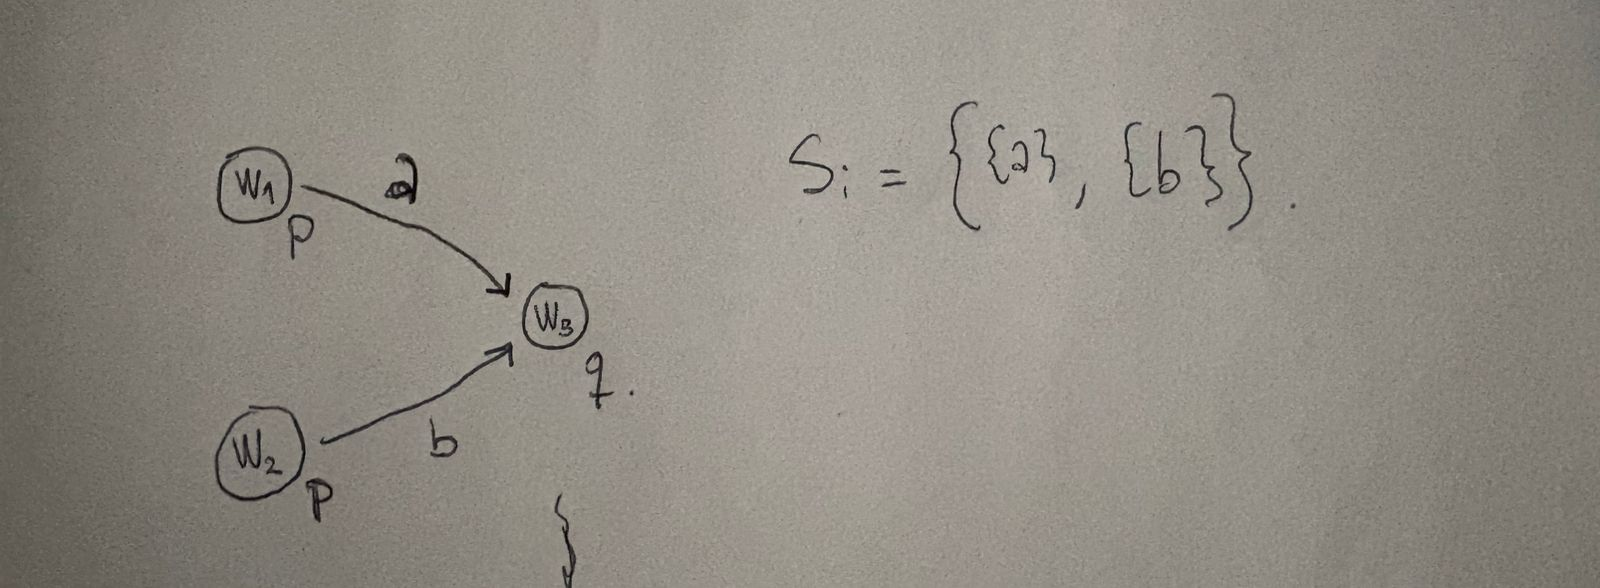
\includegraphics[width=0.5\textwidth]{imagenes/1ra_propuesta_original.jpeg}
    \caption{$\modults$}
    \label{fig:1stproposaloriginal}
\end{figure}

Con esta propuesta de contracción ($\modults'$), obtendríamos el modelo (\Cref{fig:1stproposalcontraction}):

\begin{figure}[h]
    \centering
    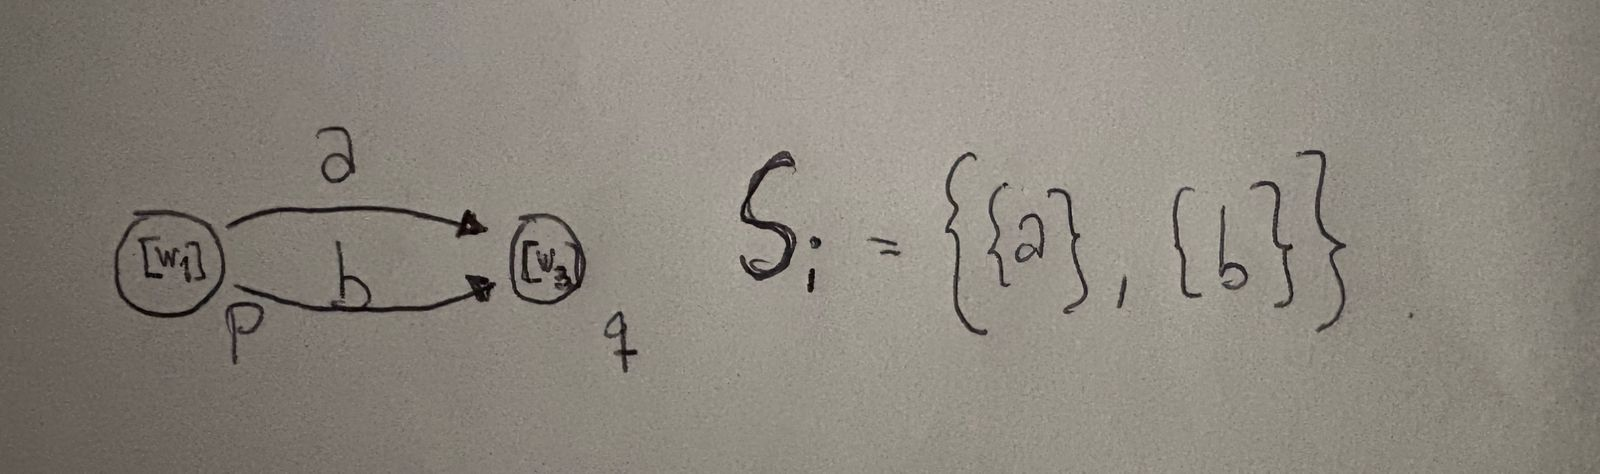
\includegraphics[width=0.5\textwidth]{imagenes/1ra_propuesta_contraido.jpeg}
    \caption{$\modults'$}
    \label{fig:1stproposalcontraction}
\end{figure}


Notemos que $\modults, w_1 \not\models \khi(p,q)$ pero $\modults', [w_1] \models \khi(p,q)$, luego $\modults,w_1$ y 
$\modults',[w_1]$ no son bisimilares.

Por lo que esta contracción por bisimulación no sería adecuada, ya que no produce un modelo bisimilar al modelo original.

Otra posible propuesta sería restringir más la relación entre las puntos del modelo contraído. Es decir, relacionar las clases 
$[w], [v] \in \rho_\modults$ cuando para cada $w' \in [w]$ existe $v' \in [v]$ tal que $w'$ y $v'$ están relacionados en el modelo original.

Luego consideremos el siguiente modelo (\Cref{fig:2ndproposaloriginal}):

\begin{figure}[h]
    \centering
    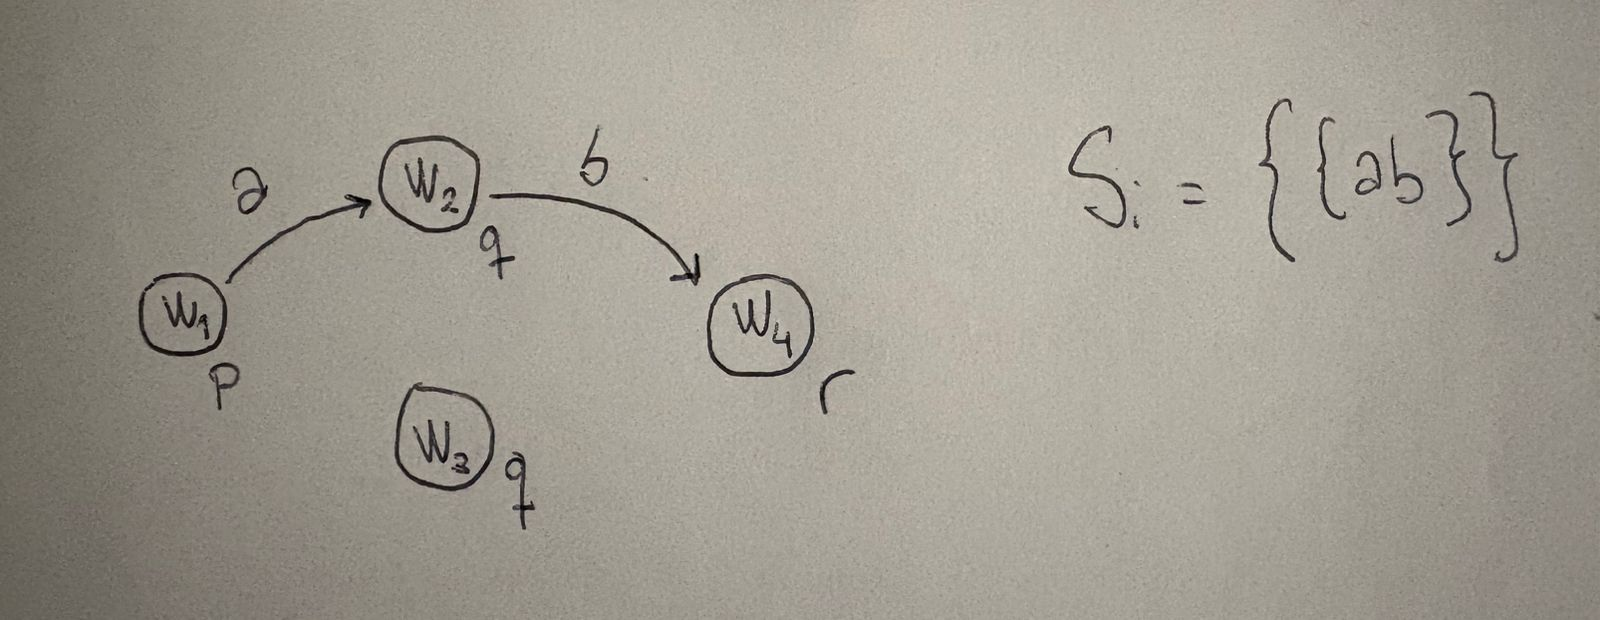
\includegraphics[width=0.5\textwidth]{imagenes/2da_propuesta_original.jpeg}
    \caption{$\modults$}
    \label{fig:2ndproposaloriginal}
\end{figure}

Y su contracción por bisimulación con la propuesta mencionada (\Cref{fig:2ndproposalcontraction}):

\begin{figure}[h]
    \centering
    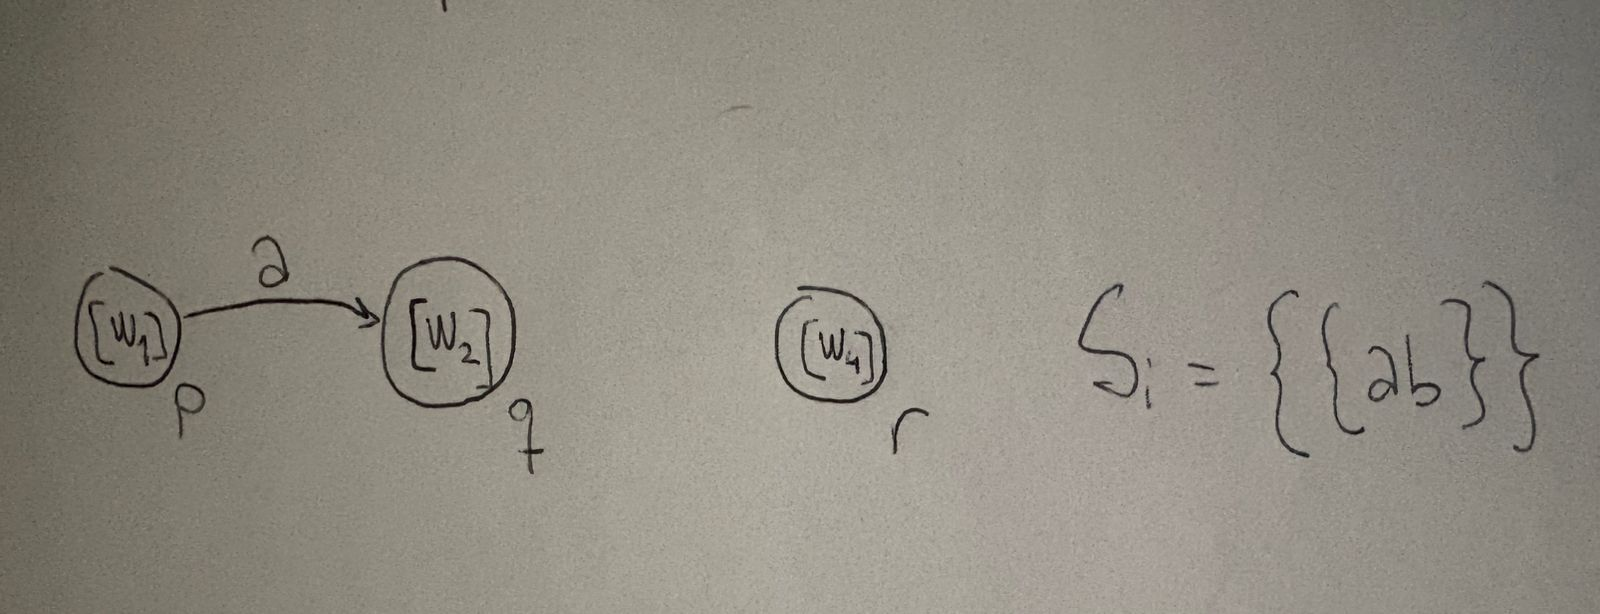
\includegraphics[width=0.5\textwidth]{imagenes/2da_propuesta_contraido.jpeg}
    \caption{$\modults'$}
    \label{fig:2ndproposalcontraction}
\end{figure}

Si analizamos ambos modelos, podemos notar que $\modults,w_1 \models \khi(p,r)$ pero $\modults',[w_1] \not\models \khi(p,r)$, luego 
$\modults,w_1$ y $\modults',[w_1]$ no son bisimilares.

Por lo que esta propuesta tampoco es adecuada, ya que tampoco produce un modelo bisimilar al modelo original.

Si analizamos ambos contraejemplos, podemos notar que la primera propuesta de contracción podría agregar caminos fuertemente ejecutables al modelo 
y la segunda podría eliminar caminos fuertemente ejecutables del modelo. Los fallos de ambas propuestas nos dan la idea de que no parece 
existir una contracción directa en la cuál no se modifique la relación de indistinguibilidad de cada agente y las acciones 
consideradas por el modelo. 

A partir de lo mencionado, surge la siguiente propuesta de contracción, la cuál modifica el conjunto de acciones y la relación de indistinguibilidad 
de cada agente.


\begin{definicion}
    Sea $\model=\tup{\W,\R,\cset{\S_i}_{i \in \AGT},\V,\ACT}$ un \ults. Se define su contracción por bisimulación, $\model'=\tup{\W',\R',\cset{\S_i'}_{i \in \AGT'},\V',\ACT'}$ donde 
    \begin{center}
        \begin{itemize}
            \item $\W' := \W/A_\modults$
            \item $\R' := \{\R'_{a_\sigma} \subseteq \W' \times \W' \mid a_\sigma \in \ACT'\}$ donde $([w],[v]) \in \R'_{a_\sigma}$ si y sólo si
            \begin{enumerate}
                \item existen $w' \in [w]$ y $v' \in [v]$ tal que $(w',v')\in \R_\sigma$
                \item $\sigma$ es fuertemente ejecutable para cada $w' \in [w]$.
            \end{enumerate}
            \item $\S_i' := \{ \pi' = \{a_\sigma \mid \sigma \in \pi\} \mid \pi \in \S_i \}$
            \item $\V'([w]) := \V(w)$
            \item $\ACT' := \{a_\sigma \mid $ existe $ \pi\in \S_i$ tal que $ \sigma \in \pi$ para algún $i \in \AGT \}$ 
        \end{itemize}
    \end{center}
\end{definicion}
    
Una vez presentada la contracción, nos gustaría asegurarnos que, efectivamente, construye un modelo bisimilar. Para ello demostraremos el 
siguiente teorema.

\begin{teorema}
    Sea $\model=\tup{\W,\R,\cset{\S_i}_{i \in \AGT},\V,\ACT}$ un \ults y sea $\modults'$ su contracción por bisimulación entonces 
    $\tup{\modults,w}$ y $\tup{\modults',[w]}$ son $\KHilogic$-bisimilares para cada $w \in \W$.
\end{teorema}

\begin{demostracion}
    Sea $\model=\tup{\W,\R,\cset{\S_i}_{i \in \AGT},\V,\ACT}$ un \ults
    y sea $\modults'$ su contracción por bisimulación, basta ver que $Z = \{(w,[w]) \in \W \times\W'\}$ es una \KHilogic-bisimulación para demostrar la propiedad.

    Dado que $\W$ es no vacío entonces es claro que $Z$ es no vacío también.

    Por otro lado, notemos que por la definición de $\V'$, es claro que $Z$ satisface (Atom).

    A su vez, por cómo definimos $Z$, es fácil ver que también (A-zig) y (A-zag) son satisfechos.
    
    Demostremos entonces que se satisfacen ($\khi$-zig) y ($\khi$-zag).

    \begin{itemize}
        \item ($\khi$-zig) Sean $U, T$ subconjuntos de $\W$ tales que $U \ultsExecAgi T$ y para cada $s \in \rho_\modults$ se cumple que 
        $s \subseteq U$ o $s \cap U = \emptyset$, queremos encontrar $T' \subseteq \W'$ que

        \begin{multicols}{2}
            \begin{itemize}
                \item $Z(U) \ultsExecAgi T'$, 
                \item $T' \subseteq Z(T)$.
            \end{itemize}
        \end{multicols}

        Veamos que $T' := \{ [w] \mid w \in T\}$ cumple con lo mencionado. Por como definimos $Z$, es claro que $T'  = Z(T)$, por lo que 
        $T' \subseteq Z(T)$. Entonces demostremos $Z(U) \ultsExecAgi T'$.

        Como $U \ultsExecAgi T$, existe $\pi \in S_i$ tal que cada plan de $\pi$ es fuertemente ejecutable en cada nodo de $U$ y 
        $\R_\pi(U) \subseteq T$. 

        Sabemos por la definición de $\modults'$ que existe $\pi' = \{a_\sigma \mid \sigma \in \pi\} \in S_i'$. Demostraremos que $\pi'$ 
        atestigua $Z(U) \ultsExecAgi T'$, es decir, que cada $a_\sigma \in \pi$ es fuertemente ejecutable en $Z(U)$ y que además 
        $\R'_{\pi'}(Z(U)) \subseteq T'$.

        Sea $[w] \in Z(U)$, veamos que $\pi'$ es fuertemente ejecutable en $[w]$. Sea $a_\sigma \in \pi'$, queremos ver que $a_\sigma$ es fuertemente 
        ejecutable en $[w]$. Notar que cómo $a_\sigma$ es un plan de un solo paso, solo basta con ver que exista $[v] \in \W'$  tal que 
        $([w],[v]) \in \R'_{a_\sigma}$.
        
        Primero notemos que como $[w] \in Z(U)$, entonces existe $w' \in [w]$ tal que $w' \in U$. Luego, por la hipótesis sobre $U$
        se cumple que $[w'] = [w] \subseteq U$. Pero veamos que como $\pi$ es fuertemente ejecutable en $U$ entonces es fuertemente ejecutable en cada nodo 
        de $[w]$, por lo que existe $v' \in \W$ tal que $v \in \R_\sigma(w')$. Como $\sigma$ es fuertemente en todo $[w]$ y $(w',v') \in \R_\sigma$, entonces 
        $([w],[v']) \in \R'_{a_\sigma}$. Queda demostrado entonces que $\pi'$ es fuertemente ejecutable en $Z(U)$.
        
        Demostraremos ahora que $\R'_{\pi'}(Z(U)) \subseteq T'$.

        Sea $[v] \in \R'_{\pi'}(Z(U))$, entonces existe $[w] \in Z(U)$ y $a_\sigma \in \pi'$ tal que $([w],[v]) \in \R'_{a_\sigma}$. Notar que 
        como $[w] \in Z(U)$, entonces existe $w' \in [w]$ tal que $w' \in U$ y, por lo tanto, $[w'] = [w] \subseteq U$. Si analizamos la definición 
        de $\R'_{a_\sigma}$, como $([w],[v]) \in \R'_{a_\sigma}$ entonces existen $w'' \in [w]$ y $v'' \in [v]$ tal que $(w'',v'') \in \R_\sigma$.
        Como $w'' \in U$ y $\R_\pi(U) \subseteq T$, entonces se cumple que $v'' \in T$, lo que nos dice que $[v''] = [v] \in T'$, que era lo que 
        queríamos demostrar. Luego $\R'_{\pi'}(Z(U)) \subseteq T'$. 

        Queda demostrado entonces que $Z$ satisface $\khi$-zig.

        \item ($\khi$-zag) Sean $U', T' \in \W'$ tales que $U' \ultsExecAgi T'$ y para cada $s \in \rho_{\modults'}$ se cumple que $s \subseteq U'$ o 
        $s \cap U' = \emptyset$, queremos encontrar $T \subseteq \W$ tal que:
        \begin{multicols}{2}
            \begin{itemize}
                \item $Z^{-1}(U') \ultsExecAgi T$, 
                \item $T \subseteq Z^{-1}(T')$.
            \end{itemize}
        \end{multicols}
        
        Veamos que $T := \bigcup\limits_{[w] \in T'} [w]$ cumple con lo mencionado. Notar que por la definición de $Z$, es claro que $T = Z^{-1}(T')$, lo que nos dice que $T \subseteq Z^{-1}(T')$. Demostremos entonces que $Z^{-1}(U') \ultsExecAgi T$. 
    
        Como $U' \ultsExecAgi T'$, entonces existe $\pi' \in \S_i'$ tal que $\pi'$ es fuertemente ejecutable para cada $[w] \in U'$ y $\R'_{\pi'}(U') \subseteq T'$.

        Luego, por como está definido $\modults$, existe $\pi \in \S_i$ tal que para cada $\sigma \in \pi$ se cumple que $a_\sigma \in \pi'$. 
        Veamos entonces que $\pi$ atestigua $Z^{-1}(U') \ultsExecAgi T$, es decir, que $\pi$ es fuertemente ejecutable para cada $w \in Z^{-1}(U')$ 
        y, a su vez, que $\R_\pi(Z^{-1}(U')) \subseteq T$.

        Sea $w \in Z^{-1}(U')$, veamos que $\pi$ es fuertemente ejecutable en $w$. Sea $\sigma \in \pi$, queremos ver que $\sigma$ es fuertemente ejecutable 
        en $w$. Notemos que como $w \in Z^{-1}(U')$ entonces $[w] \in U'$ y, a su vez, como $a_\sigma$ es fuertemente ejecutable en $U'$, $a_\sigma$ también es fuertemente ejecutable en $[w]$. 
        Luego, existe $[v]$ tal que $([w],[v]) \in \R'_{a_\sigma}$. Notemos que por la definición de $\R'$, como existe esa arista entonces se cumple que $\sigma$ es fuertemente ejecutable 
        para cada nodo de $[w]$. En particular, $\sigma$ es fuertemente ejecutable en $w$, lo que demuestra que $\pi$ es fuertemente ejecutable 
        en $Z^{-1}(U')$.

        Demostremos ahora que $\R_{\pi}(Z^{-1}(U')) \subseteq T'$. 

        Sean $w, v \in \W$ tales que $w \in Z^{-1}(U')$ y $(w,v) \in \R_\pi$, queremos ver que $v \in T'$. Primero veamos que como $(w,v) \in \R_\pi$, 
        entonces existe $\sigma \in \pi$ tal que $(w,v) \in \R_\sigma$. Luego, como $w \in Z^{-1}(U')$, entonces $[w] \in U'$. Como $\pi'$ es fuertemente 
        ejecutable en $U'$, entonces $a_\sigma$ es fuertemente ejecutable en $U'$ y, por lo tanto, $a_\sigma$ también es fuertemente ejecutable en $[w]$.
        
        Pero, como $a_\sigma$ es fuertemente ejecutable en $[w]$ entonces existe $[v']$ tal que $([w],[v']) \in \R_{a_\sigma}$. 
        Como existe dicha arista, por la definición de $\R'$, ocurre que $\sigma$ es fuertemente ejecutable en todo nodo de $[w]$. 
        Luego, como $\sigma$ es fuertemente ejecutable en todo nodo de $[w]$ y $(w,v) \in \R_\sigma$ entonces $([w],[v]) \in \R'_{a_\sigma}$. 
        Luego, como $\R'_{\pi'}(U') \subseteq T'$, entonces $[v] \in T'$, lo que nos dice que $v \in T$ que era lo que queríamos demostrar.

        Entonces, hemos demostrado que $Z$ satisface $\khi$-zag.
    \end{itemize}
    Demostramos que $Z$ es una \KHilogic-bisimulación. Luego $\tup{\modults,w}$ y $\tup{\modults',[w]}$ son $\KHilogic$-bisimilares para cada $w \in \W$.
\end{demostracion}


% \begin{teorema}
%     La contracción por bisimulación de un \ults $\modults$ tiene cardinalidad mínima entre los modelos $\KHilogic$-bisimilares a $\modults$.
% \end{teorema}
Hemos demostrado entonces que la contracción propuesta es adecuada, es decir, que dado un \ults genera un \ults bisimilar a partir de su 
autobisimulación máxima $A_\modults$.

Luego, es deseable que la contracción propuesta sea razonable en términos computacionales. Por lo que demostraremos el siguiente teorema.


\begin{teorema}
    Sea $\modults$ un \ults, computar su contracción por bisimulación $\modults'$ es realizable en tiempo polinomial en el 
    tamaño de $\modults$.
\end{teorema}

\begin{demostracion}
    Veamos que el tamaño de $\modults'$ es polinomial con respecto al tamaño de $\modults$. Es claro que $W/A_\modults$ tiene tamaño polinomial con 
    respecto al tamaño de $\W$ y lo mismo sucede con $\V'$. 

    Luego notemos que $\ACT'$ tiene tamaño $\sum_{i} |\S_i|$, y cada $\S_i'$ tiene tamaño a lo sumo $|\S_i|$. Por último, notemos que $\R'$ tiene a lo 
    sumo una arista por cada tupla formada por dos nodos de $\W$ y un plan conocido por algún agente $i$, luego su tamaño está acotado por 
    $\W * \W * \sum_{i}|\S_i|$, lo cuál es polinomial con respecto al tamaño de $\modults$.

    Una vez demostrado que el tamaño de $\modults'$ es polinomial con respecto al tamaño de $\modults$, basta con ver que cada componente es computable en 
    tiempo polinomial. 

    Es claro que las componentes $\W'$, $\{\S_i'\}$, $\V'$ y $\ACT'$ son computables en tiempo polinomial. Luego notemos que como mencionamos en 
    (sección complejidad marco teórico), model-checking está en $\Poly$ por lo que es claro que computar $\sexec(\sigma)$ y $\R_\sigma$
    para cada $\sigma$ es realizable en tiempo polinomial. 

    Luego $\modults'$ es computable en tiempo polinomial.
\end{demostracion}

Hemos presentado una contracción por bisimulación para la lógica de `Knowing How' multi-agente basada en incertidumbre y hemos demostrado que 
la misma es adecuada, es decir, que produce un modelo bisimilar y que además es computable eficientemente.

Sin embargo, algo que podemos notar a partir de la definición propuesta, es que el modelo que se encuentra difiere estructuralmente de 
forma signicativa con respecto al modelo original. 
Naturalmente, al modificar el conjunto de acciones básicas del modelo, el entorno de habilidades de los agentes cambia por completo y, junto con ello, 
los planes que cada agente considera posible y su relación de indistinguibilidad cambian también. Más aún, en la contracción propuesta, los agentes 
únicamente consideran planes de una única acción.

Este análisis es el que motiva una nueva propuesta de contracción.

\section{Segunda Propuesta de Contracción}

Como mencionamos en la sección anterior, queremos encontrar una contracción que produzca un modelo bisimilar al modelo original pero que conserve 
en la mayor medida sus características estructurales. En particular, sería deseable que mantenga el conjunto de acciones básicas y la relación de 
indistinguibilidad de planes de cada agente.

Si recordamos las primeras propuestas analizadas en la sección anterior, notamos que no logramos encontrar una propuestra adecuada a partir de 
la autobisimulación máxima $A_\modults$ que no modifique las componentes mencionadas. Por lo que pareciera que para encontrar tal contracción 
debemos considerar otro dominio.  

Notemos que cada \ults de la forma $\model=\tup{\W,\R,\cset{\S_i}_{i \in \AGT},\V,\ACT}$ tiene naturalmente un modelo de Kripke asociado, 
que sería el formado por $\tup{\W,\{\R_a\}_{a\in\ACT},\V}$. Luego, una posible propuesta sería contraer dicho modelo de Kripke como en 
Lógica Modal Básica y utilizarlo como contracción para `Knowing-How' conservando el conjunto de acciones básicas y la relación de indistinguibilidad 
de planes de cada agente. 

\begin{definicion}
    Supongamos $\ACT$ un conjunto de acciones no vacío enumerable.
    Sea $\modults = \tup{\W,\{\R_a\}_{a\in\ACT},\V}$ un modelo de Kripke. Sea $Z_\modults$ su autobisimulación máxima en Lógica Modal Básica (LMB) entonces definimos su contracción por LMB-bisimulación como $\modults_{LMB} = \tup{\W',\{\R'_a\}_{a\in\ACT},\V'}$ donde
    \begin{center}
        \begin{itemize}
            \item $\W' := \W /Z_\modults$
            \item $\R_a' := \{([w],[v]) \mid$ existen $w' \in [w]$ y $v' \in [v]$ tal que $(w',v') \in \R_a \}$
            \item $\V'([w]) := \V(w)$
        \end{itemize}
    \end{center} 
\end{definicion}

Notar que en el contexto de esta sección, al escribir $[w]$ nos referiremos a la clase de equivalencia de $w$ en la relación de 
equivalencia dada por $Z_\modults$.

\begin{lema}\label{lema:LMB-R-lema}
    Sea $\model = \tup{\W,\{\R_a\}_{a\in\ACT},\V}$ un modelo de Kripke, y sea $\modults_{LMB} = \tup{\W',\{\R_a'\}_{a\in\ACT},\V'}$ su contracción por LMB-bisimulación.
    Si $([w],[v]) \in \R'_a$ entonces para cada $w' \in [w]$ existe $v' \in [v]$ tal que $(w',v') \in \R_a$
\end{lema}

\begin{demostracion}
    Sea $\model = \tup{\W,\{\R_a\}_{a\in\ACT},\V}$ un modelo de Kripke, y sea $\modults_{LMB} = \tup{\W',\{\R_a'\}_{a\in\ACT},\V'}$ su contracción por LMB-bisimulación. Sea $([w],[v]) \in \R'_a$, veamos que para cada $w' \in [w]$ existe $v' \in [v]$ tal que $(w',v') \in \R_a$.

    Como $([w],[v]) \in \R'_a$ existen $w_0 \in [w]$ y $v_0 \in [v]$ tales que $(w_0,v_0)\in \R_a$. Sea $w' \in [w]$, por estar ambos 
    $w_0$ y $w'$ en $[w]$, existe una LMB-bisimulación $Z$ tal que $(w_0,w') \in Z$. Pero notemos que, por (zig) de $Z$, como 
    $(w_0,v_0) \in \R_a$  entonces existe $v'$ tal que $(w',v') \in \R_a$ y, a su vez, 
    $(v_0,v') \in Z$, es decir, $v' \in [v]$, que era lo que queríamos demostrar.
\end{demostracion}

Ahora, una vez presentada la contracción por LMB-bisimulación, demostraremos el siguiente teorema que extiende dicha contracción para 
la lógica `Knowing How' multi-agente basada en incertidumbre.

\begin{teorema}
    Sea $\model=\tup{\W,\R,\cset{\S_i}_{i \in \AGT},\V,\ACT}$ un \ults y $\modults_{LMB} = \tup{\W',\{\R_a'\}_{a\in\ACT},\V'}$ 
    la contracción por LMB-bisimulación del modelo de Kripke $\tup{\W,\{\R_a\}_{a\in\ACT},\V}$, entonces $\tup{\modults,w}$ y $\tup{\modults',[w]}$ 
    son $\KHilogic$-bisimilares para cada $w \in \W$ siendo $\modults' = \tup{\W',\R',\cset{\S_i}_{i \in \AGT},\V',\ACT}$.
\end{teorema}

Notar que en este teorema, al fijar $\model=\tup{\W,\R,\cset{\S_i}_{i \in \AGT},\V,\ACT}$ inmediatamente fijamos a $\ACT$ como el conjunto no vacío enumerable de acciones para la Lógica Modal Básica.

\begin{demostracion}
    Queremos ver que $Z = \{(w,[w]) \mid w \in \W\}$ es una \KHilogic-bisimulación.
    
    Por definición de la contracción por bisimulación en (LMB) se puede ver que se satisface (Atom). Luego, por definición de Z, es fácil ver que (A-zig) y (A-zag) son satisfechas. Demostremos entonces ($\khi$-zig) y ($\khi$-zag).

    \begin{itemize}
        \item ($\khi$-zig). Sean $U, T \subseteq \W$ tales que $U \ultsExecAgi T$ y para cada $s \in \rho_\modults$ se cumple $s \subseteq U$ o 
        $s \cap U = \emptyset$. Queremos ver que existe $T' \subseteq \W'$ tal que

        \begin{multicols}{2}
            \begin{itemize}
                \item $Z(U) \ultsExecAgi T'$, 
                \item $T' \subseteq Z(T)$.
            \end{itemize}
        \end{multicols}
        Veamos que $T' := \{[w] \mid w \in T\}$ cumple con lo mencionado. Notemos que $T' = Z(T)$, por lo que solo debemos demostrar 
        $Z(U) \ultsExecAgi T'$.

        Como $U \ultsExecAgi T$, existe $\pi \in S_i$ tal que $\pi$ es fuertemente ejecutable en $U$ y a su vez $\R_\pi(U) \subseteq T$.

        Demostremos que $\pi$ es fuertemente ejecutable en $Z(U)$ y que $\R'_\pi(Z(U)) \subseteq T'$.

        Supongamos que $\pi$ no es fuertemente ejecutable en $Z(U)$. Luego existe $\sigma \in \pi$ y $[w_1],...,[w_k]$ 
        con $1 \le k \le |\sigma|$ tal que $[w_1] \in Z(U)$, $([w_i], [w_{i+1}]) \in \R'_{\sigma[i]}$ y 
        $\R'_{\sigma[k]}([w_k]) = \emptyset$.

        Como $[w_1] \in Z(U)$, existe $w_1' \in U$ tal que $w_1' \in [w_1]$. Luego notemos que aplicando sucesivamente el \Cref{lema:LMB-R-lema} 
        en todo el camino, existen $w_1',...w_k'$ tales que $w_i' \in [w_i]$ y $(w_i',w_{i+1}') \in \R_{\sigma[i]}$.

        Pero veamos que esto nos dice que $\R_{\sigma[k]}(w_k') = \emptyset$. Pues, si existiera $v$ tal que 
        $(w_k',v) \in \R_{\sigma[k]}$ entonces ocurriría que $([w_k],[v]) \in \R'_{\sigma[k]}$. Luego $\sigma \in \pi$ no es 
        fuertemente ejecutable en $w_1' \in U$, lo cuál es absurdo, pues dijimos que $\pi$ es fuertemente ejecutable en todo $U$.

        Veamos ahora que $\R'_\pi(Z(U)) \subseteq T'$.

        Sea $[v] \in \R'_\pi(Z(U))$, entonces existen $\sigma \in \pi$ y $[w_1], ..., [w_{|\sigma|+1}]$ tales que 
        $[w_1] \in Z(U)$, $([w_i],[w_{i+1}]) \in \R'_{\sigma[i]}$ y $[w_{|\sigma|+1}] = [v]$.

        Como $[w_1] \in Z(U)$, entonces existe $w_1' \in U$ tal que $w_1'\in [w_1]$. Luego, notemos que aplicando sucesivamente el 
        \Cref{lema:LMB-R-lema} sobre el camino, existen $w_1',...,w_{|\sigma|+1}'$ tales que $w_i' \in [w_i]$ y $(w_i',w_{i+1}')\in \R_{\sigma[i]}$. 
        Como $\R_\pi(U) \subseteq T$ esto nos dice que $w'_{|\sigma|+1} \in T$. Por definición de 
        $T'$, $[w_{|\sigma|+1}] \in T'$. Finalmente, como $[v] = [w_{|\sigma|+1}]$ entonces $[v] \in T'$.

        Luego, demostramos que $\pi$ es fuertemente ejecutable en $Z(U)$ y que $\R'_\pi(Z(U)) \subseteq T'$. 
        Juntando ambos resultados, concluimos que $Z(U) \ultsExecAgi T'$, lo cuál demuestra ($\khi$-zig).

       \item ($\khi$-zag) Sean $U', T' \subseteq \W'$ tales que $U' \ultsExecAgi T'$ y para cada $s \in \rho_{\modults'}$ se cumple $s \subseteq U'$ o 
        $s \cap U' = \emptyset$. Queremos ver que existe $T \subseteq \W$ tal que

       \begin{multicols}{2}
            \begin{itemize}
                \item $Z^{-1}(U') \ultsExecAgi T$, 
                \item $T \subseteq Z^{-1}(T')$.
            \end{itemize}
        \end{multicols}

        Veamos que $T = \{w \mid [w] \in T'\}$ cumple con lo mencionado. Notemos que $T = Z^{-1}(T')$, por lo que solo debemos demostrar 
        $Z^{-1}(U') \ultsExecAgi T$.

        Como $U' \ultsExecAgi T'$, existe $\pi \in \S_i$ tal que $\pi$ es fuertemente ejecutable en todo $U'$ y a su vez 
        $\R'_\pi(U') \subseteq T'$.

        Veamos que $\pi$ es fuertemente ejecutable para cada $w \in Z^{-1}(U')$ y que $\R_\pi(Z^{-1}(U')) \subseteq T$.

        Supongamos que $\pi$ no es fuertemente ejecutable en $w \in Z^{-1}(U')$. Luego, existe $\sigma \in \pi$ y $w_1,...,w_k$ con 
        $1 \le k \le |\sigma|$ tal que $w_1 = w$, $(w_i,w_{i+1}) \in \R_{\sigma[i]}$ y $\R_{\sigma[k]}(w_k) = \emptyset$. 

        Notemos entonces que por la definición de $\R'$, $[w_1],...,[w_k]$ cumple que $([w_i],[w_{i+1}]) \in \R'_{\sigma[i]}$ y, a su vez, 
        que $[w_1] \in U'$, pues $w_1 \in Z^{-1}(U')$. Pero, como $\pi$ es fuertemente ejecutable en $U'$, entonces $\sigma$ también lo es, por lo que 
        existe $[v]$ tal que $([w_k],[v]) \in \R'_{\sigma[k]}$. Lo cuál nos lleva a un absurdo, pues si ese fuera el caso entonces por 
        \Cref{lema:LMB-R-lema} tendríamos que existe $v' \in [v]$ tal que $(w_k,v') \in \R_{\sigma[k]}$ pero habíamos dicho que 
        $\R_{\sigma[k]}(w_k) = \emptyset$.

        Esto nos dice que $\pi$ es fuertemente ejecutable para cada $w \in Z^{-1}(U')$.

        Veamos ahora que $\R_\pi(Z^{-1}(U')) \subseteq T$.

        Sea $v \in \R_\pi(Z^{-1}(U'))$, entonces existen $\sigma \in \pi$ y $w_1,...,w_{|\sigma|+1}$ tales que 
        $w_1 \in Z^{-1}(U')$, $(w_i,w_{i+1}) \in \R_{\sigma[i]}$ y $w_{|\sigma|+1} = v$. 

        Por la definición de $\R'$, esto nos dice que $[w_1],...,[w_{|\sigma|+1}]$ cumple que $([w_i],[w_{i+1}]) \in \R'_{\sigma[i]}$ 
        y, a su vez, como $w_1 \in Z^{-1}(U')$ entonces $[w_1] \in U'$. Luego notemos que como $\R'_\pi(U') \subseteq T'$, esto nos dice que 
        $[w_{|\sigma|+1}] \in T'$, lo cuál implica que $w_{|\sigma|+1} \in T$. Como $v = w_{|\sigma|+1}$ entonces $v \in T$. 

        Entonces demostramos que $\pi$ es fuertemente ejecutable para cada $w \in Z^{-1}(U')$ y que $\R'_\pi(Z^{-1}(U')) \subseteq T$. 
        Juntando ambos resultados, concluimos que $Z^{-1}(U') \ultsExecAgi T$, lo cuál demuestra ($\khi$-zag).
    \end{itemize}
    Demostramos entonces que $Z$ es una \KHilogic-bisimulación. Luego $\tup{\modults,w}$ y $\tup{\modults',[w]}$ son $\KHilogic$-bisimilares 
    para cada $w \in \W$.
\end{demostracion}

Un punto muy positivo de esta contracción es que existen algoritmos eficientes que computan la contracción por LMB-bisimulación. En particular, 
el algoritmo de Paige y Tarjan presentado en \cite[`Partición Relacional más Gruesa']{Paige&TarjanContraction} tiene complejidad $\bigO(m*log(n))$ siendo $n$ la cantidad de nodos del dominio del modelo y 
$m$ la cantidad de aristas del mismo.


\section{Comparación entre las contracciones propuestas}


Acá irían ejemplos donde cada contracción genere un modelo de menor tamaño. También conclusiones acerca de lo que nos dice sobre expresividad cada
contracción.

% \section{Ideas sueltas}
\begin{teorema}
    Sea $\model_=\tup{\W,\R,\cset{\S_i}_{i \in \AGT},\V,\ACT}$ un modelo, y sea $Z \subseteq \W \times \W$ una relación binaria que satisface (atom) y $Id := \{(w,w)\in \W\} \subseteq Z$, entonces $Z$ es una autobisimulación.
\end{teorema}

No se si dice mucho este teorema, pero al menos caracteriza un poco las autobisimulaciones.

Resumen de lo trabajado:

\begin{itemize}

\item Primera sección: Contracción por bisimulación

Conclusiones positivas acerca de las contracciones, nos dicen cosas sobre la expresividad de la lógica, en el sentido de que demostramos que dado un modelo siempre existe otro en el que la función de valuación es inyectiva (no hay dos nodos que satisfagan exactamente el mismo conjunto de variables proposicionales), usa planes de solo un paso y las clases de equivalencia de planes que conoce cada agente son simplemente singletons y aún así la lógica no sabe cómo diferenciarlos (son lógicamente equivalentes).

También, logramos contraer un modelo a otro donde chequear strong executability se logra en un solo paso, por lo que potencialmente se ahorra cómputo al no necesitar cada paso intermedio de un plan.

Ambas contracciones son computables en tiempo polinomial en el tamaño del modelo lo cuál es muy bueno.


Conclusiones negativas, no logramos encontrar una contracción que de verdad minimice el \rm\textbf{tamaño} del modelo en cuestión. Si bien, seguro encontramos un modelo lógicamente equivalente que minimiza la cantidad de nodos, puede darse el caso que la contracción aumente considerablemente la cantidad de aristas (sin embargo, hay que considerar el trade-off del ahorro en el chequeo de strong executability).

Cosas a analizar: 
\begin{itemize}
    \item Hay una contracción mejor?
    \item Puede tener que ver la definición de bisimulación con el hecho de que no encontramos una contracción totalmente convincente (ver teorema de esta sección capaz)? 
    \item Como dijo Carlos, puede tener que ver con la naturaleza de los modelos donde se interpreta la lógica? En ese caso considerar hacer un análisis desde teoría de modelos.
\end{itemize}


\item Segunda sección: Bisimulación entre dos modelos

Queda escribir el algoritmo para demostrar membership y revisar la demo de hardness para confirmar que la reducción está efectivamente bien.

Creo que este problema queda bastante completo una vez hechas esas dos cosas.

\end{itemize}


\bibliographystyle{plain}
\bibliography{referencias}


\end{document}

